% Encoder and decoder of the local-sla-16yr AnemoiModelEncProcDec.
%
%   page 1  the encoder wire diagram, drawn entirely in symbols
%   page 2  the processor wire diagram
%   page 3  the decoder wire diagram, same block vocabulary
%   page 4  the notation table, with the values read out of the checkpoint
%   page 5  notes -- what this configuration is doing
%   page 6  candidates for architectural experimentation
%   page 7  comparison with the DeepMind lineage (runs onto page 8)
%
% Build:  make            (regenerates dims.tex / symbols_table.tex first)
%         latexmk -pdf network_diagram.tex
%
% To drop the figure alone into a paper, % ---------------------------------------------------------------------------
% Encoder of AnemoiModelEncProcDec (GraphTransformerForwardMapper), drawn at the
% block level of "Attention Is All You Need" Fig. 1, with every wire annotated
% by its array shape.
%
% The tikzpicture only -- \input it into a document whose preamble loads
% notation.tex and the tikz libraries listed in network_diagram.tex.
%
% Layout: three lanes flowing left to right --
%   DATA   (top)     x-space nodes:  psi -> Linear -> LayerNorm -> key, value
%   EDGE   (middle)  encoder edges:  a_e -> Linear -> eps
%   LATENT (bottom)  z-space nodes:  a_z -> Linear -> LayerNorm -> query, self
% converging at the graph attention block, after which the latent stream
% continues alone along the middle line.
%
% Every node is placed off the \row*/\col* registers below, so the figure is
% reflowed by editing numbers in one place rather than by moving nodes.
% ---------------------------------------------------------------------------

% --- lane (row) positions ---------------------------------------------------
\def\rowdata{0}          % data-space lane
\def\rowedge{-6.0}       % edge lane; also the latent stream after attention
\def\rowlat{-12.0}        % latent-space lane
\def\rowbypass{4.2}      % raw psi running over the top to the decoder
\def\rowconn{-9.0}       % graph connectivity entering the attention block
\def\rowselfskip{-16.0}  % self branch routed under the attention block
\def\rowdstskip{-18.6}   % pre-norm latent skip routed under everything
\def\rowffskip{-3.0}     % skip around the feed forward

% --- column positions -------------------------------------------------------
\def\colA{0}        % inputs
\def\colcat{4.8}    % concatenation
\def\colB{7.7}      % embedding Linear
\def\colC{11.4}     % LayerNorm
\def\colD{15.4}     % q / k / v / edge projections
\def\colsplit{13.4} % where a LayerNorm output branches in two
\def\colE{21.6}     % graph attention
\def\colF{26.6}     % residual 1
\def\colG{29.4}     % projection
\def\colH{32.6}     % residual 2
\def\colI{35.6}     % LayerNorm + feed forward
\def\colJ{38.6}     % residual 3
\def\colK{40.8}     % output

\def\stack{1.15}    % vertical offset of paired sub-boxes

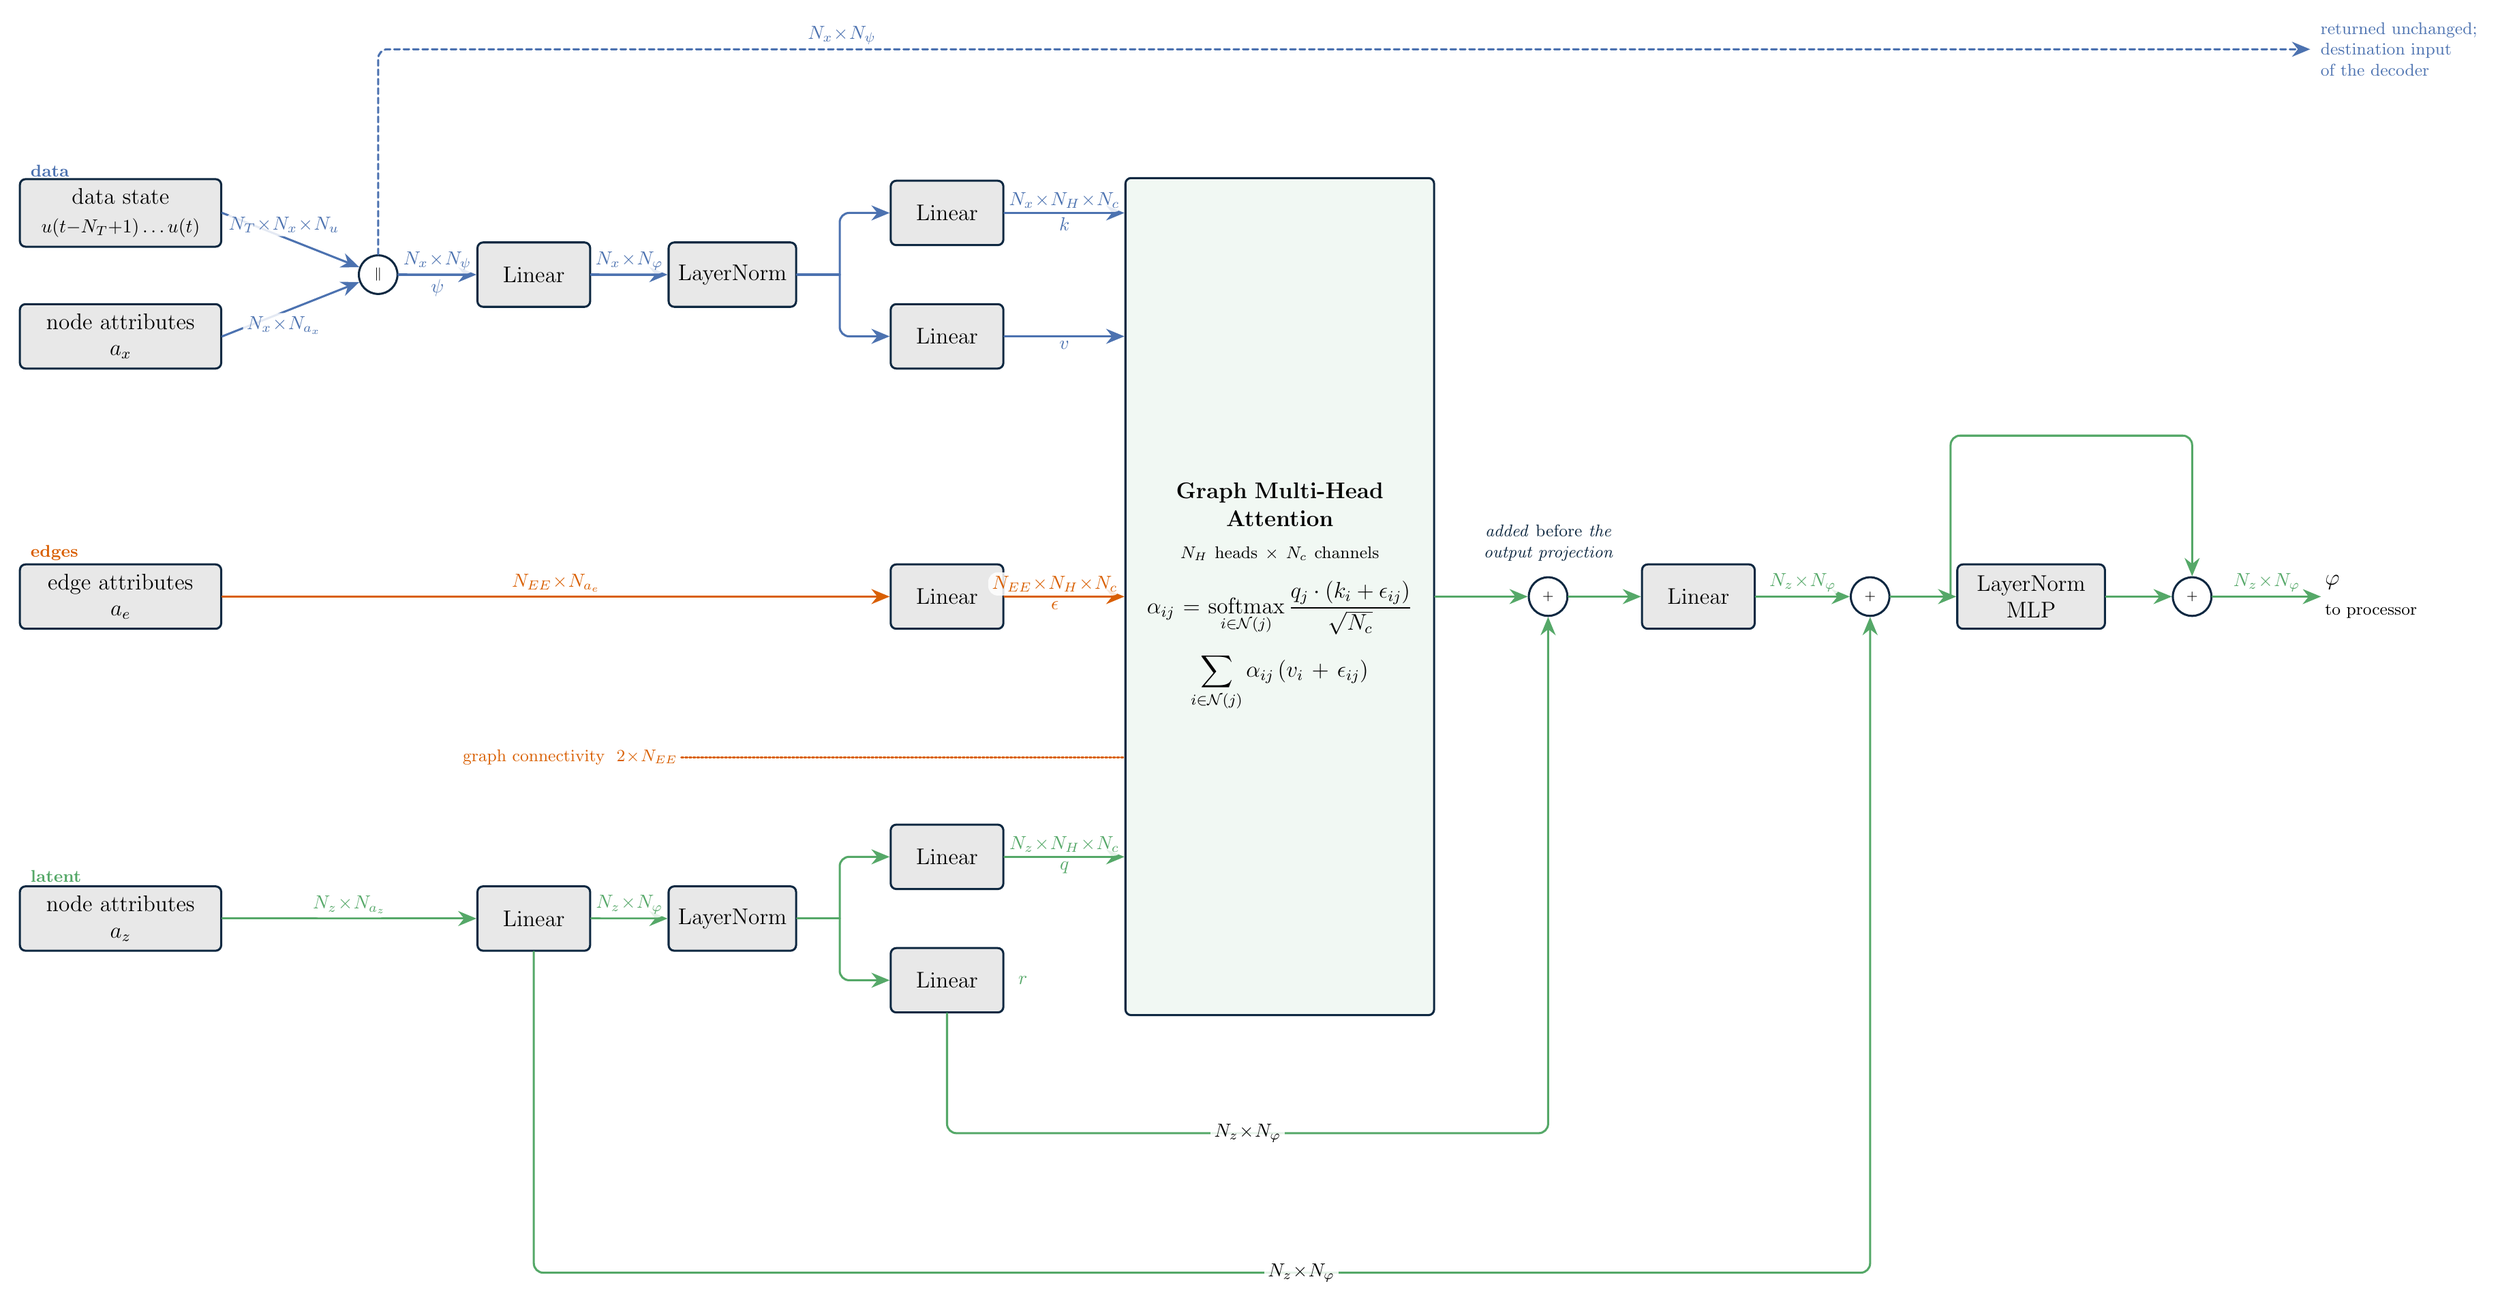
\begin{tikzpicture}[
  x=1cm, y=1cm, font=\large,
  blk/.style     = {rounded corners=3pt, draw=trapline, fill=trapfill,
                    line width=1.1pt, align=center, inner sep=5pt,
                    minimum height=1.2cm, minimum width=2.1cm},
  attnblk/.style = {blk, fill=attnfill},
  sum/.style     = {circle, draw=trapline, fill=white, line width=1.1pt,
                    inner sep=0pt, minimum size=0.72cm},
  term/.style    = {align=center, inner sep=2pt},
  wire/.style    = {-{Stealth[length=3.4mm,width=2.8mm]}, line width=1.1pt,
                    line cap=round, rounded corners=5pt},
  plain/.style   = {line width=1.1pt, line cap=round, rounded corners=5pt},
  shp/.style     = {font=\normalsize, inner sep=2pt, fill=white,
                    fill opacity=0.85, text opacity=1},
  tag/.style     = {font=\normalsize\itshape, inner sep=2pt},
  lane/.style    = {font=\small\bfseries, anchor=south west},
]

% =========================== lane labels ====================================
% anchored on the left edge of the input boxes so nothing overhangs the
% bounding box (the standalone crop would clip it)
\node[lane, text=dataclr]   at ({\colA-1.8}, {\rowdata+\stack+0.55}) {data};
\node[lane, text=edgeclr]   at ({\colA-1.8}, {\rowedge+0.55})        {edges};
\node[lane, text=latentclr] at ({\colA-1.8}, {\rowlat+0.55})         {latent};

% =========================== DATA LANE ======================================
\node[blk, text width=3.4cm] (uin)  at (\colA, {\rowdata+\stack})
  {data state\\[1pt]{\normalsize$\datavec(t{-}\NT{+}1)\dots\datavec(t)$}};
\node[blk, text width=3.4cm] (axin) at (\colA, {\rowdata-\stack})
  {node attributes\\$\attrx$};
\node[sum] (cat)  at (\colcat, \rowdata) {\scriptsize$\|$};
\node[blk] (embx) at (\colB, \rowdata) {Linear};
\node[blk] (lnx)  at (\colC, \rowdata) {LayerNorm};
\node[blk] (link) at (\colD, {\rowdata+1.15}) {Linear};
\node[blk] (linv) at (\colD, {\rowdata-1.15}) {Linear};
\coordinate (xsplit) at (\colsplit, \rowdata);

\draw[wire, dataclr] (uin.east)  -- node[shp, above, pos=0.45]
  {\shapethree{\NT}{\Nx}{\Nu}} (cat);
\draw[wire, dataclr] (axin.east) -- node[shp, below, pos=0.45]
  {\shapetwo{\Nx}{\Nax}} (cat);
\draw[wire, dataclr] (cat) -- node[shp, above] {\shapetwo{\Nx}{\Npsi}}
                             node[tag, below, text=dataclr] {$\inputvec$} (embx);
\draw[wire, dataclr] (embx) -- node[shp, above] {\shapetwo{\Nx}{\Nphi}} (lnx);
\draw[plain, dataclr] (lnx.east) -- (xsplit);
\draw[wire, dataclr] (xsplit) |- (link.west);
\draw[wire, dataclr] (xsplit) |- (linv.west);

% the mapper returns its source input untouched; it is the decoder's dst input
\draw[wire, dataclr, densely dashed] (cat.north) |- (\colK, \rowbypass)
  node[shp, above, pos=0.62] {\shapetwo{\Nx}{\Npsi}}
  node[term, anchor=west, xshift=3pt, align=left, font=\small]
  {returned unchanged;\\destination input\\of the decoder};

% =========================== EDGE LANE ======================================
\node[blk, text width=3.4cm] (aein) at (\colA, \rowedge)
  {edge attributes\\$\attre$};
\node[blk] (line) at (\colD, \rowedge) {Linear};
\node[term, anchor=west, align=left, font=\small, text=edgeclr,
      fill=white, inner sep=2pt] (conn)
  at ({\colB-1.4}, \rowconn) {graph connectivity\ \ $2\!\times\!\NEE$};

\draw[wire, edgeclr] (aein) -- node[shp, above] {\shapetwo{\NEE}{\Nae}} (line);

% =========================== LATENT LANE ====================================
\node[blk, text width=3.4cm] (azin) at (\colA, \rowlat)
  {node attributes\\$\attrz$};
\node[blk] (embz) at (\colB, \rowlat) {Linear};
\node[blk] (lnz)  at (\colC, \rowlat) {LayerNorm};
\node[blk] (linq) at (\colD, {\rowlat+1.15}) {Linear};
\node[blk] (lins) at (\colD, {\rowlat-1.15}) {Linear};
\coordinate (zsplit) at (\colsplit, \rowlat);

\draw[wire, latentclr] (azin) -- node[shp, above] {\shapetwo{\Nz}{\Naz}} (embz);
\draw[wire, latentclr] (embz) -- node[shp, above] {\shapetwo{\Nz}{\Nphi}} (lnz);
\draw[plain, latentclr] (lnz.east) -- (zsplit);
\draw[wire, latentclr] (zsplit) |- (linq.west);
\draw[wire, latentclr] (zsplit) |- (lins.west);

% =========================== ATTENTION ======================================
\node[attnblk, minimum height=15.6cm, text width=5.4cm] (attn) at (\colE, \rowedge)
  {\textbf{Graph Multi-Head}\\[1pt]\textbf{Attention}\\[3pt]
   {\small $\NH$ heads $\times$ $\Nc$ channels}\\[10pt]
   {\large$\displaystyle
      \attn_{ij}=\operatorname*{softmax}_{i\in\nbhd(j)}
      \frac{\query_j\cdot(\keyv_i+\edgeemb_{ij})}{\sqrt{\Nc}}$}\\[9pt]
   {\large$\displaystyle
      \sum_{i\in\nbhd(j)}\attn_{ij}\,(\valuev_i+\edgeemb_{ij})$}};

\draw[wire, dataclr] (link.east) -- node[shp, above]
  {\shapethree{\Nx}{\NH}{\Nc}} node[tag, below, text=dataclr] {$\keyv$}
  (link.east -| attn.west);
\draw[wire, dataclr] (linv.east) -- node[tag, below, text=dataclr] {$\valuev$}
  (linv.east -| attn.west);
\draw[wire, edgeclr] (line.east) -- node[shp, above, pos=0.42]
  {\shapethree{\NEE}{\NH}{\Nc}} node[tag, below, pos=0.42, text=edgeclr] {$\edgeemb$}
  (line.east -| attn.west);
\draw[wire, latentclr] (linq.east) -- node[shp, above]
  {\shapethree{\Nz}{\NH}{\Nc}} node[tag, below, text=latentclr] {$\query$}
  (linq.east -| attn.west);
\draw[plain, edgeclr, densely dotted] (conn.east) -- (conn.east -| attn.west);

% =========================== POST-ATTENTION CHAIN ===========================
\node[sum] (res1) at (\colF, \rowedge) {\scriptsize$+$};
\node[blk] (proj) at (\colG, \rowedge) {Linear};
\node[sum] (res2) at (\colH, \rowedge) {\scriptsize$+$};
\node[blk, text width=2.4cm] (ff) at (\colI, \rowedge)
  {LayerNorm\\MLP};
\node[sum] (res3) at (\colJ, \rowedge) {\scriptsize$+$};
\node[term, anchor=west, align=left] (out) at ({\colK+0.2}, \rowedge)
  {$\latentvec$\\[2pt]{\small to processor}};

\draw[wire, latentclr] (attn.east) -- (res1);
\draw[wire, latentclr] (res1) -- (proj);
\node[tag, above=6pt of res1, text=trapline, align=center]
  {\small added \emph{before} the\\[-1pt]\small output projection};
\draw[wire, latentclr] (proj) -- node[shp, above] {\shapetwo{\Nz}{\Nphi}} (res2);
\draw[wire, latentclr] (res2) -- (ff);
\draw[wire, latentclr] (ff) -- (res3);
\draw[wire, latentclr] (res3) -- node[shp, above] {\shapetwo{\Nz}{\Nphi}} (out);


% residual 1 -- the self branch, added in attention space, ahead of the
% output projection (AIAYN draws that projection inside its attention box)
\draw[wire, latentclr] (lins.south) |- ({\colF}, \rowselfskip) -- (res1.south);
\node[shp] at ({(\colD+\colF)/2}, \rowselfskip) {\shapetwo{\Nz}{\Nphi}};
\node[tag, anchor=west, text=latentclr]
  at ({\colD+1.25}, {\rowlat-1.15}) {$\selfv$};

% residual 2 -- pre-norm skip taken from the latent embedding
\draw[wire, latentclr] (embz.south) |- ({\colH}, \rowdstskip) -- (res2.south);
\node[shp] at ({(\colC+\colH)/2}, \rowdstskip) {\shapetwo{\Nz}{\Nphi}};

% residual 3 -- pre-norm skip around the MLP
\draw[wire, latentclr] ({(\colH+\colI)/2}, \rowedge) |- ({\colJ}, \rowffskip)
  -- (res3.north);

\end{tikzpicture}
 inside a
% tikzpicture-capable preamble, or use the standalone build: make figure.

\documentclass[11pt,landscape]{article}
\usepackage[a4paper,landscape,margin=1.2cm]{geometry}
\usepackage[T1]{fontenc}
\usepackage{amsmath}
\usepackage{amssymb}
\usepackage{array}
\usepackage{booktabs}
\usepackage{multicol}
\usepackage{enumitem}
\usepackage{tikz}
\usetikzlibrary{arrows.meta, positioning, calc, fit}

% Fonts: plain Latin Modern by default.  To match a preprint built on
% preprint.sty (as figures/nested-illustration does), swap in:
%     \usepackage{XCharter}
%     \usepackage[charter,smallerops]{newtxmath}

% --- palette ---------------------------------------------------------------
% Structural greys from the pptx theme used in nested_illustration.tex; one
% accent per lane from the notebooks/nice.mplstyle prop_cycle.
\definecolor{trapfill}{HTML}{E8E8E8}
\definecolor{trapline}{HTML}{0E2841}
\definecolor{dataclr}{HTML}{4C72B0}
\definecolor{edgeclr}{HTML}{D95F02}
\definecolor{latentclr}{HTML}{55A868}
% A fourth accent, used only for the decoder's output extractor and the output
% channels, so the one thing the decoder page exists to show is the one thing not
% drawn in a lane colour.
\definecolor{diagclr}{HTML}{8172B2}
\colorlet{diagfill}{diagclr!8}
\colorlet{inactiveclr}{black!45}
\colorlet{attnfill}{latentclr!8}

% Symbol macros for the network diagrams.
%
% Convention: lowercase for variables and functions; uppercase is reserved for
% matrices, except for integer counts, which are always N_{quantity}.
%
% This is the ONE place a symbol is renamed -- the figure, the notation table and
% any caption all pick the change up.  Numbers live in dims.tex (generated).

% --- data space --------------------------------------------------------------
\newcommand{\coordx}{x}                 % data-space node coordinate
\newcommand{\Nx}{N_{x}}                 % number of data-space nodes
\newcommand{\datavec}{u}                % data features at one timestep
\newcommand{\Nu}{N_{u}}                 % number of data features per timestep
\newcommand{\NT}{N_{T}}                 % number of input timesteps
\newcommand{\attrx}{a_{x}}              % data-node attributes
\newcommand{\Nax}{N_{a_{x}}}
\newcommand{\inputvec}{\psi}            % assembled data-node input
\newcommand{\Npsi}{N_{\psi}}

% --- latent space ------------------------------------------------------------
\newcommand{\coordz}{z}                 % latent-space node coordinate
\newcommand{\Nz}{N_{z}}                 % number of latent-space nodes
\newcommand{\attrz}{a_{z}}              % latent-node attributes
\newcommand{\Naz}{N_{a_{z}}}
\newcommand{\latentvec}{\varphi}        % latent state vector
\newcommand{\Nphi}{N_{\varphi}}         % number of latent channels

% --- graph edges -------------------------------------------------------------
% The encoder and decoder graphs are distinct edge sets with distinct attributes
% and distinct weights; only the widths happen to coincide, so one symbol serves
% both and the edge counts carry the distinction.
\newcommand{\attre}{a_{e}}              % edge attributes
\newcommand{\Nae}{N_{a_{e}}}
\newcommand{\NEE}{N_{EE}}               % encoder edges, data -> latent
\newcommand{\NDE}{N_{DE}}               % decoder edges, latent -> data
\newcommand{\nbhd}{\mathcal{N}}         % incoming neighbourhood of a destination node

% --- model output ------------------------------------------------------------
\newcommand{\outvec}{y}                 % model output in data space
\newcommand{\Nout}{N_{y}}               % number of output channels
\newcommand{\idxprog}{\mathcal{P}}      % prognostic output channels
\newcommand{\idxdiag}{\mathcal{D}}      % diagnostic output channels
% Counts of the two, so the sets keep the set symbols and the integer counts are
% written N_{quantity} like every other count here.  Subscripting the set macro
% means renaming a set renames its count with it.
\newcommand{\Nprog}{N_{\idxprog}}
\newcommand{\Ndiag}{N_{\idxdiag}}

% --- attention ---------------------------------------------------------------
\newcommand{\NH}{N_{H}}                 % attention heads
\newcommand{\Nc}{N_{c}}                 % channels per head, N_phi / N_H
\newcommand{\query}{q}
\newcommand{\keyv}{k}
\newcommand{\valuev}{v}
\newcommand{\edgeemb}{\epsilon}         % embedded edge attributes
\newcommand{\selfv}{r}                  % lin_self branch
\newcommand{\attn}{\alpha}

% --- mlp ---------------------------------------------------------------------
% anemoi's own name for this block (cf. the mlp_hidden_ratio config knob)
\newcommand{\ff}{f}                     % the MLP
\newcommand{\Nf}{N_{f}}                 % MLP hidden width

% --- shape annotation --------------------------------------------------------
% One macro so the styling of every wire label changes in one place.
\newcommand{\shape}[1]{\ensuremath{#1}}
\newcommand{\shapetwo}[2]{\shape{#1 \!\times\! #2}}
\newcommand{\shapethree}[3]{\shape{#1 \!\times\! #2 \!\times\! #3}}

% Literal values for the DeepMind lineage (GraphCast, GenCast, FGN / WeatherNext 2).
%
% *** HAND-MAINTAINED.  This is the one \newcommand file here that is NOT
% *** generated -- dims.tex and symbols_table.tex come out of extract_dims.py and
% *** are overwritten by make.  These numbers describe someone else's models, so
% *** no checkpoint of ours can produce them; the discipline that survives is
% *** that they live in exactly one place and each one carries its source.
%
% Provenance matters more than usual here, because the three models' papers,
% their shipped configs and their released checkpoints disagree in places:
%
%   [P] stated in the paper
%   [C] only in a shipped config file in the repo
%   [K] only recoverable by decoding a released checkpoint
%   [D] derived arithmetic (mesh construction, BFS on the mesh), not quoted anywhere
%
% Traps worth remembering, all of them hit while collecting these:
%   * google-deepmind/graphcast was RENAMED to google-deepmind/weathernext (same
%     repo id, old URLs 301-redirect, old graphcast/*.py paths 404).  All three
%     models now live in one tree -- weathernext1_graph/, weathernext1_gen/,
%     weathernext2/ -- over a shared utils/.  GenCast and FGN import the same
%     utils/sparse_transformer.py.
%   * GenCast's paper D.3 gives 41162 mesh nodes / 246960 edges where the code
%     produces 40962 / 245760.  The code is unambiguous; the paper looks like a
%     typo.  We quote the code.
%   * The demo notebooks' random-init defaults (attention_k_hop 16, mesh_size 4)
%     are NOT the paper models.  Do not read hyperparameters off a notebook.
%   * GraphCast's radius_query_fraction_edge_length appears in the paper and in
%     the demo notebook but never in library code.

% --- shared across the lineage -----------------------------------------------
\newcommand{\dmradiusfrac}{0.6}          % [P] GraphCast S3.3 fn.5; [K] GenCast ckpts; [C] WN2.json
\newcommand{\dmradiuskm}{79}             % [D] 0.6 x longest level-6 edge, chord, on a unit sphere
\newcommand{\dmmeshnodes}{40{,}962}      % [D] level-6 icosahedral mesh; contradicts GenCast D.3
\newcommand{\dmmeshlevel}{6}             % [P] all three
\newcommand{\dmdecdeg}{3}                % [C] in_mesh_triangle_indices, containing face

% --- GraphCast ----------------------------------------------------------------
\newcommand{\gclatent}{512}              % [P] S3.7
\newcommand{\gcsteps}{16}                % [P] S3.5, unshared weights
\newcommand{\gcparams}{36.7}             % [P] main text, millions
\newcommand{\gcencdeg}{39.5}             % [D] 1{,}618{,}746 G2M edges [P] / 40962 mesh nodes
\newcommand{\gcmeshlevels}{0--6}         % [P] S3.5, merged into one multimesh

% --- GenCast (denoiser core) --------------------------------------------------
\newcommand{\genlatent}{512}             % [K] released checkpoint
\newcommand{\genlayers}{16}              % [K][P] D.3
\newcommand{\genheads}{4}                % [K]
\newcommand{\genheaddim}{128}            % [K] 512/4; the splash kernel asserts a multiple of 128
\newcommand{\genffw}{2048}               % [K] 4 x d_model
\newcommand{\genkhop}{32}                % [K] checkpoint, corroborated by [P] D.3
\newcommand{\genparams}{57}              % [P] quoted in the FGN paper, millions
\newcommand{\genballnodes}{3{,}169}      % [D] BFS, 1+3k(k+1) for a degree-6 node
\newcommand{\gendensity}{7.7}            % [D] 3169/40962, per cent
\newcommand{\genballkm}{900}             % [D] 32 hops x ~28 km mean level-6 edge
\newcommand{\genaggnorm}{16}             % [K] grid2mesh_aggregate_normalization
\newcommand{\gennoisedim}{16}            % [K] noise_encoder output_sizes (32, 16)

% --- FGN / WeatherNext 2 ------------------------------------------------------
\newcommand{\fgnlatent}{768}             % [C] WeatherNext2.json; [P] A.3
\newcommand{\fgnlayers}{24}              % [C][P] A.3
\newcommand{\fgnheads}{6}                % [C][P] A.3
\newcommand{\fgnffw}{3072}               % [C] 4 x d_model
\newcommand{\fgnkhop}{32}                % [C] ONLY -- the FGN paper never mentions the sparsity
\newcommand{\fgnparams}{180}             % [P] Sec. 2.3, millions
\newcommand{\fgnedgewidth}{32}           % [C][P] A.3, cut down from GenCast's 512
\newcommand{\fgnaggnorm}{4}              % [C] aggregate_normalization
\newcommand{\fgnnoisedim}{32}            % [C][P] A.3, the FiLM conditioning vector
\newcommand{\fgnfilmlayers}{57}          % [D] count over the config; 49 of them in the processor
\newcommand{\fgnheaddim}{128}            % [C] key_size / value_size, unchanged from GenCast

% GENERATED by extract_dims.py -- do not edit.
% source: ../../runs/v4/checkpoint/23c396bfc6ff4049a776ee6aca7af43f/inference-last.ckpt
% dataset: ocean
% date: 2026-09-08

\newcommand{\valNx}{33469}
\newcommand{\valNz}{12288}
\newcommand{\valNax}{4}
\newcommand{\valNaz}{4}
\newcommand{\valNu}{35}
\newcommand{\valNpsi}{109}
\newcommand{\valNphi}{128}
\newcommand{\valNH}{4}
\newcommand{\valNc}{32}
\newcommand{\valNae}{3}
\newcommand{\valNf}{512}
\newcommand{\valNEE}{107950}
\newcommand{\valNDE}{100407}
\newcommand{\valNout}{1}
\newcommand{\valNL}{4}
\newcommand{\valNw}{512}
\newcommand{\valNchunk}{4}
\newcommand{\valNprog}{0}
\newcommand{\valNdiag}{1}
\newcommand{\valdiagnamesplain}{sla}
\newcommand{\valdiagnames}{{\tt sla}}
\newcommand{\valNaxtrain}{0}
\newcommand{\valNaztrain}{0}
\newcommand{\valNaetrain}{0}
\newcommand{\valencparams}{230272}
\newcommand{\valdecparams}{230017}
\newcommand{\valprocparams}{791552}
\newcommand{\valproclayerparams}{197888}
\newcommand{\valnodeparams}{0}
\newcommand{\valedgeparams}{0}
\newcommand{\valgraphparams}{0}
\newcommand{\valtotalparams}{1251841}
\newcommand{\valgraphpct}{0}
\newcommand{\valdegmin}{0}
\newcommand{\valdegmax}{15}
\newcommand{\valdegmean}{8.8}
\newcommand{\valdegzero}{2967}
\newcommand{\valdecdegmin}{3}
\newcommand{\valdecdegmax}{3}
\newcommand{\valdecdegmean}{3.0}
\newcommand{\valdecdegzero}{0}
\newcommand{\valwindowlat}{11}
\newcommand{\valwindowreach}{22}
\newcommand{\valringordered}{1}
\newcommand{\valenccutoffkm}{200}
\newcommand{\valhiddenspacing}{204}
\newcommand{\valcutoffratio}{1.0}
\newcommand{\valwindowfrac}{8.3}
\newcommand{\valtotalparamsM}{1.25}
\newcommand{\valNT}{3}

% GENERATED by extract_dims.py -- do not edit.
% source: ../../runs/v4/checkpoint/23c396bfc6ff4049a776ee6aca7af43f/inference-last.ckpt
% dataset: ocean
% date: 2026-09-08

\newcommand{\valNaxsplit}{4}
\newcommand{\valNazsplit}{4}
\newcommand{\valNaesplit}{3}
\newcommand{\valNcsplit}{$128/4 = 32$}
\newcommand{\valNfsplit}{$4\Nphi = 512$}
\newcommand{\valdecdegphrase}{holds exactly 3 latent nodes}
\newcommand{\valtrainabletrail}{}
\newcommand{\valtrainablenote}{Every {\tt trainable\_size} is currently zero, so the node and edge attributes are purely geometric and no parameter is pinned to an individual node or edge.}

\newcommand{\symbolrowsone}{%
$\coordx$ & data-space node coordinate & -- \\
$\Nx$ & number of data-space nodes & \valNx \\
$\datavec$ & data feature vector at one timestep & -- \\
$\Nu$ & number of data features per timestep & \valNu \\
$\NT$ & number of input timesteps ({\tt multistep\_input}) & \valNT \\
$\attrx$ & data-node attributes (sin/cos lat-lon\valtrainabletrail) & -- \\
$\Nax$ & width of $\attrx$ & \valNaxsplit \\
$\inputvec$ & assembled data-node input, $\inputvec = [\datavec_{t-\NT+1},\,\dots,\,\datavec_{t},\,\attrx]$ & -- \\
$\Npsi$ & width of $\inputvec$, $\NT\Nu + \Nax$ & \valNpsi \\
$\coordz$ & latent-space node coordinate & -- \\
$\Nz$ & number of latent-space nodes & \valNz \\
$\attrz$ & latent-node attributes (sin/cos lat-lon\valtrainabletrail) & -- \\
$\Naz$ & width of $\attrz$ & \valNazsplit \\
$\latentvec$ & latent state vector & -- \\
$\Nphi$ & number of latent channels ({\tt num\_channels}) & \valNphi \\
}

\newcommand{\symbolrowstwo}{%
$\outvec$ & model output in data space & -- \\
$\Nout$ & number of output channels, $\Nout = \Nprog + \Ndiag$ & \valNout \\
$\Nprog$ & number of prognostic output channels ($\idxprog$) & \valNprog \\
$\Ndiag$ & number of diagnostic output channels ($\idxdiag$) & \valNdiag \\
$\attre$ & edge attributes (length, direction\valtrainabletrail) & -- \\
$\Nae$ & width of $\attre$ & \valNaesplit \\
$\NEE$ & number of encoder edges (data $\to$ latent) & \valNEE \\
$\NDE$ & number of decoder edges (latent $\to$ data) & \valNDE \\
$\nbhd(\coordz_j)$ & data-space nodes with an edge into latent node $\coordz_j$ & -- \\
$\nbhd(\coordx_j)$ & latent-space nodes with an edge into data node $\coordx_j$ & -- \\
$\NH$ & number of attention heads & \valNH \\
$\Nc$ & channels per head, $\Nc = \Nphi/\NH$ & \valNcsplit \\
$\ff$ & MLP, $\ff:\mathbb{R}^{\Nphi}\to\mathbb{R}^{\Nphi}$, GELU & -- \\
$\Nf$ & MLP hidden width ({\tt mlp\_hidden\_ratio}) & \valNfsplit \\
}


\pagestyle{empty}

\begin{document}

% ============================== page 1 =====================================
\vspace*{\fill}
\begin{center}
  \resizebox{\textwidth}{!}{% ---------------------------------------------------------------------------
% Encoder of AnemoiModelEncProcDec (GraphTransformerForwardMapper), drawn at the
% block level of "Attention Is All You Need" Fig. 1, with every wire annotated
% by its array shape.
%
% The tikzpicture only -- \input it into a document whose preamble loads
% notation.tex and the tikz libraries listed in network_diagram.tex.
%
% Layout: three lanes flowing left to right --
%   DATA   (top)     x-space nodes:  psi -> Linear -> LayerNorm -> key, value
%   EDGE   (middle)  encoder edges:  a_e -> Linear -> eps
%   LATENT (bottom)  z-space nodes:  a_z -> Linear -> LayerNorm -> query, self
% converging at the graph attention block, after which the latent stream
% continues alone along the middle line.
%
% Every node is placed off the \row*/\col* registers below, so the figure is
% reflowed by editing numbers in one place rather than by moving nodes.
% ---------------------------------------------------------------------------

% --- lane (row) positions ---------------------------------------------------
\def\rowdata{0}          % data-space lane
\def\rowedge{-6.0}       % edge lane; also the latent stream after attention
\def\rowlat{-12.0}        % latent-space lane
\def\rowbypass{4.2}      % raw psi running over the top to the decoder
\def\rowconn{-9.0}       % graph connectivity entering the attention block
\def\rowselfskip{-16.0}  % self branch routed under the attention block
\def\rowdstskip{-18.6}   % pre-norm latent skip routed under everything
\def\rowffskip{-3.0}     % skip around the feed forward

% --- column positions -------------------------------------------------------
\def\colA{0}        % inputs
\def\colcat{4.8}    % concatenation
\def\colB{7.7}      % embedding Linear
\def\colC{11.4}     % LayerNorm
\def\colD{15.4}     % q / k / v / edge projections
\def\colsplit{13.4} % where a LayerNorm output branches in two
\def\colE{21.6}     % graph attention
\def\colF{26.6}     % residual 1
\def\colG{29.4}     % projection
\def\colH{32.6}     % residual 2
\def\colI{35.6}     % LayerNorm + feed forward
\def\colJ{38.6}     % residual 3
\def\colK{40.8}     % output

\def\stack{1.15}    % vertical offset of paired sub-boxes

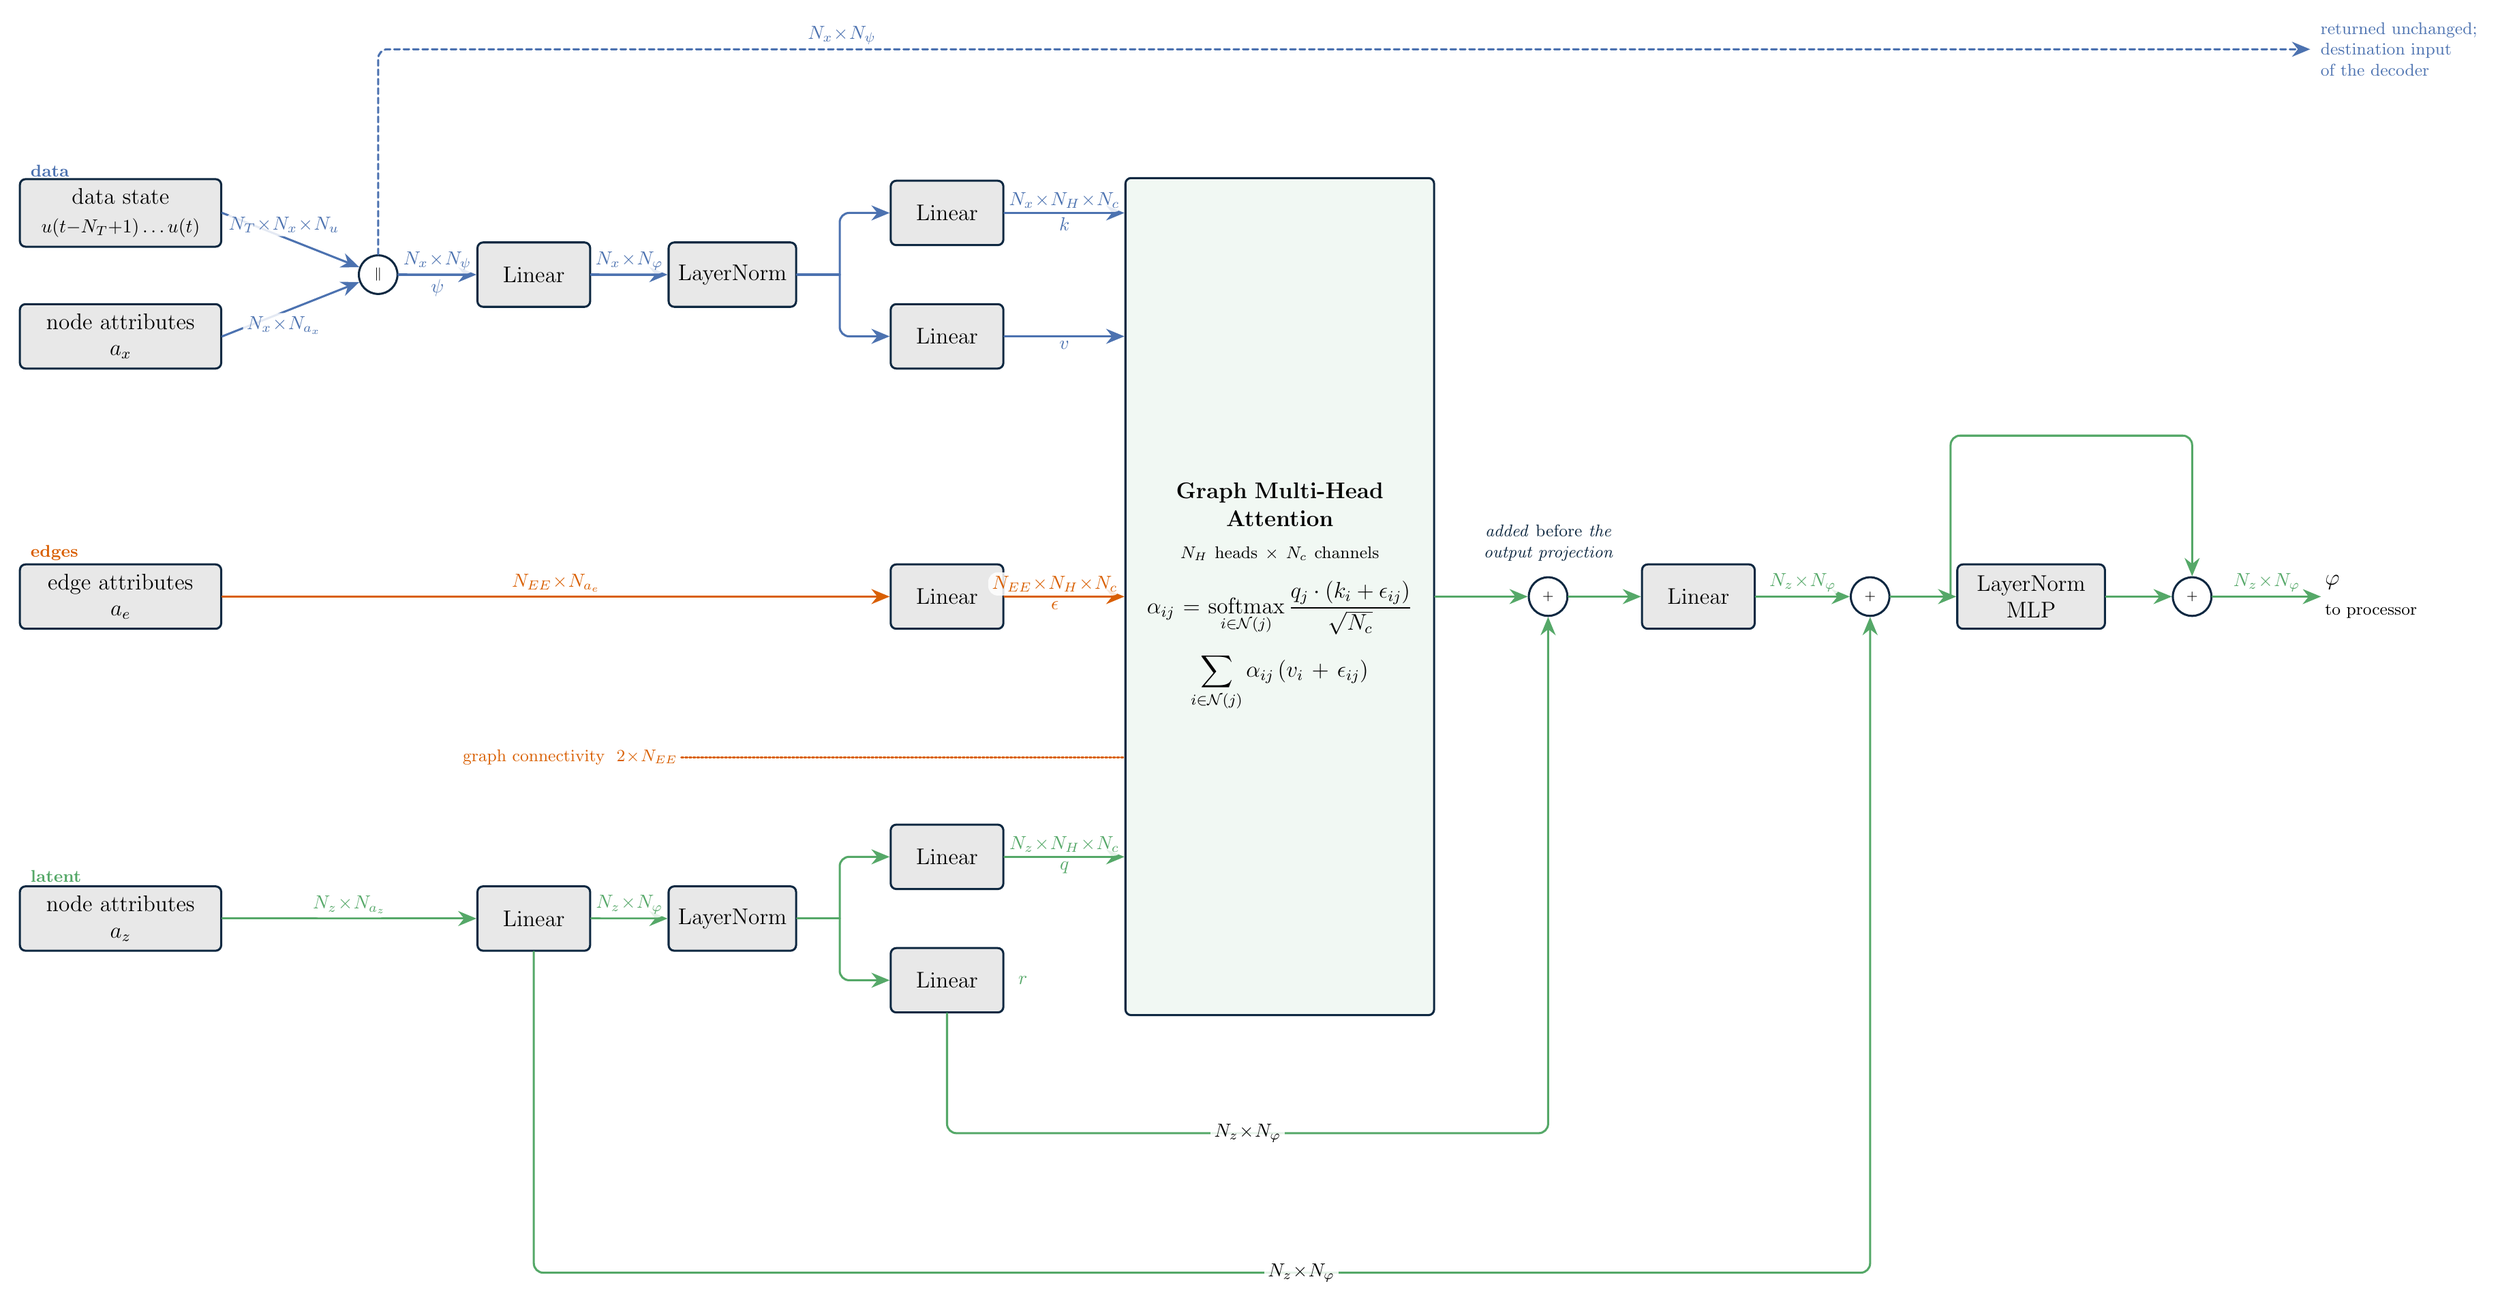
\begin{tikzpicture}[
  x=1cm, y=1cm, font=\large,
  blk/.style     = {rounded corners=3pt, draw=trapline, fill=trapfill,
                    line width=1.1pt, align=center, inner sep=5pt,
                    minimum height=1.2cm, minimum width=2.1cm},
  attnblk/.style = {blk, fill=attnfill},
  sum/.style     = {circle, draw=trapline, fill=white, line width=1.1pt,
                    inner sep=0pt, minimum size=0.72cm},
  term/.style    = {align=center, inner sep=2pt},
  wire/.style    = {-{Stealth[length=3.4mm,width=2.8mm]}, line width=1.1pt,
                    line cap=round, rounded corners=5pt},
  plain/.style   = {line width=1.1pt, line cap=round, rounded corners=5pt},
  shp/.style     = {font=\normalsize, inner sep=2pt, fill=white,
                    fill opacity=0.85, text opacity=1},
  tag/.style     = {font=\normalsize\itshape, inner sep=2pt},
  lane/.style    = {font=\small\bfseries, anchor=south west},
]

% =========================== lane labels ====================================
% anchored on the left edge of the input boxes so nothing overhangs the
% bounding box (the standalone crop would clip it)
\node[lane, text=dataclr]   at ({\colA-1.8}, {\rowdata+\stack+0.55}) {data};
\node[lane, text=edgeclr]   at ({\colA-1.8}, {\rowedge+0.55})        {edges};
\node[lane, text=latentclr] at ({\colA-1.8}, {\rowlat+0.55})         {latent};

% =========================== DATA LANE ======================================
\node[blk, text width=3.4cm] (uin)  at (\colA, {\rowdata+\stack})
  {data state\\[1pt]{\normalsize$\datavec(t{-}\NT{+}1)\dots\datavec(t)$}};
\node[blk, text width=3.4cm] (axin) at (\colA, {\rowdata-\stack})
  {node attributes\\$\attrx$};
\node[sum] (cat)  at (\colcat, \rowdata) {\scriptsize$\|$};
\node[blk] (embx) at (\colB, \rowdata) {Linear};
\node[blk] (lnx)  at (\colC, \rowdata) {LayerNorm};
\node[blk] (link) at (\colD, {\rowdata+1.15}) {Linear};
\node[blk] (linv) at (\colD, {\rowdata-1.15}) {Linear};
\coordinate (xsplit) at (\colsplit, \rowdata);

\draw[wire, dataclr] (uin.east)  -- node[shp, above, pos=0.45]
  {\shapethree{\NT}{\Nx}{\Nu}} (cat);
\draw[wire, dataclr] (axin.east) -- node[shp, below, pos=0.45]
  {\shapetwo{\Nx}{\Nax}} (cat);
\draw[wire, dataclr] (cat) -- node[shp, above] {\shapetwo{\Nx}{\Npsi}}
                             node[tag, below, text=dataclr] {$\inputvec$} (embx);
\draw[wire, dataclr] (embx) -- node[shp, above] {\shapetwo{\Nx}{\Nphi}} (lnx);
\draw[plain, dataclr] (lnx.east) -- (xsplit);
\draw[wire, dataclr] (xsplit) |- (link.west);
\draw[wire, dataclr] (xsplit) |- (linv.west);

% the mapper returns its source input untouched; it is the decoder's dst input
\draw[wire, dataclr, densely dashed] (cat.north) |- (\colK, \rowbypass)
  node[shp, above, pos=0.62] {\shapetwo{\Nx}{\Npsi}}
  node[term, anchor=west, xshift=3pt, align=left, font=\small]
  {returned unchanged;\\destination input\\of the decoder};

% =========================== EDGE LANE ======================================
\node[blk, text width=3.4cm] (aein) at (\colA, \rowedge)
  {edge attributes\\$\attre$};
\node[blk] (line) at (\colD, \rowedge) {Linear};
\node[term, anchor=west, align=left, font=\small, text=edgeclr,
      fill=white, inner sep=2pt] (conn)
  at ({\colB-1.4}, \rowconn) {graph connectivity\ \ $2\!\times\!\NEE$};

\draw[wire, edgeclr] (aein) -- node[shp, above] {\shapetwo{\NEE}{\Nae}} (line);

% =========================== LATENT LANE ====================================
\node[blk, text width=3.4cm] (azin) at (\colA, \rowlat)
  {node attributes\\$\attrz$};
\node[blk] (embz) at (\colB, \rowlat) {Linear};
\node[blk] (lnz)  at (\colC, \rowlat) {LayerNorm};
\node[blk] (linq) at (\colD, {\rowlat+1.15}) {Linear};
\node[blk] (lins) at (\colD, {\rowlat-1.15}) {Linear};
\coordinate (zsplit) at (\colsplit, \rowlat);

\draw[wire, latentclr] (azin) -- node[shp, above] {\shapetwo{\Nz}{\Naz}} (embz);
\draw[wire, latentclr] (embz) -- node[shp, above] {\shapetwo{\Nz}{\Nphi}} (lnz);
\draw[plain, latentclr] (lnz.east) -- (zsplit);
\draw[wire, latentclr] (zsplit) |- (linq.west);
\draw[wire, latentclr] (zsplit) |- (lins.west);

% =========================== ATTENTION ======================================
\node[attnblk, minimum height=15.6cm, text width=5.4cm] (attn) at (\colE, \rowedge)
  {\textbf{Graph Multi-Head}\\[1pt]\textbf{Attention}\\[3pt]
   {\small $\NH$ heads $\times$ $\Nc$ channels}\\[10pt]
   {\large$\displaystyle
      \attn_{ij}=\operatorname*{softmax}_{i\in\nbhd(j)}
      \frac{\query_j\cdot(\keyv_i+\edgeemb_{ij})}{\sqrt{\Nc}}$}\\[9pt]
   {\large$\displaystyle
      \sum_{i\in\nbhd(j)}\attn_{ij}\,(\valuev_i+\edgeemb_{ij})$}};

\draw[wire, dataclr] (link.east) -- node[shp, above]
  {\shapethree{\Nx}{\NH}{\Nc}} node[tag, below, text=dataclr] {$\keyv$}
  (link.east -| attn.west);
\draw[wire, dataclr] (linv.east) -- node[tag, below, text=dataclr] {$\valuev$}
  (linv.east -| attn.west);
\draw[wire, edgeclr] (line.east) -- node[shp, above, pos=0.42]
  {\shapethree{\NEE}{\NH}{\Nc}} node[tag, below, pos=0.42, text=edgeclr] {$\edgeemb$}
  (line.east -| attn.west);
\draw[wire, latentclr] (linq.east) -- node[shp, above]
  {\shapethree{\Nz}{\NH}{\Nc}} node[tag, below, text=latentclr] {$\query$}
  (linq.east -| attn.west);
\draw[plain, edgeclr, densely dotted] (conn.east) -- (conn.east -| attn.west);

% =========================== POST-ATTENTION CHAIN ===========================
\node[sum] (res1) at (\colF, \rowedge) {\scriptsize$+$};
\node[blk] (proj) at (\colG, \rowedge) {Linear};
\node[sum] (res2) at (\colH, \rowedge) {\scriptsize$+$};
\node[blk, text width=2.4cm] (ff) at (\colI, \rowedge)
  {LayerNorm\\MLP};
\node[sum] (res3) at (\colJ, \rowedge) {\scriptsize$+$};
\node[term, anchor=west, align=left] (out) at ({\colK+0.2}, \rowedge)
  {$\latentvec$\\[2pt]{\small to processor}};

\draw[wire, latentclr] (attn.east) -- (res1);
\draw[wire, latentclr] (res1) -- (proj);
\node[tag, above=6pt of res1, text=trapline, align=center]
  {\small added \emph{before} the\\[-1pt]\small output projection};
\draw[wire, latentclr] (proj) -- node[shp, above] {\shapetwo{\Nz}{\Nphi}} (res2);
\draw[wire, latentclr] (res2) -- (ff);
\draw[wire, latentclr] (ff) -- (res3);
\draw[wire, latentclr] (res3) -- node[shp, above] {\shapetwo{\Nz}{\Nphi}} (out);


% residual 1 -- the self branch, added in attention space, ahead of the
% output projection (AIAYN draws that projection inside its attention box)
\draw[wire, latentclr] (lins.south) |- ({\colF}, \rowselfskip) -- (res1.south);
\node[shp] at ({(\colD+\colF)/2}, \rowselfskip) {\shapetwo{\Nz}{\Nphi}};
\node[tag, anchor=west, text=latentclr]
  at ({\colD+1.25}, {\rowlat-1.15}) {$\selfv$};

% residual 2 -- pre-norm skip taken from the latent embedding
\draw[wire, latentclr] (embz.south) |- ({\colH}, \rowdstskip) -- (res2.south);
\node[shp] at ({(\colC+\colH)/2}, \rowdstskip) {\shapetwo{\Nz}{\Nphi}};

% residual 3 -- pre-norm skip around the MLP
\draw[wire, latentclr] ({(\colH+\colI)/2}, \rowedge) |- ({\colJ}, \rowffskip)
  -- (res3.north);

\end{tikzpicture}
}
\end{center}
\vspace*{\fill}

{\footnotesize
    \textbf{Encoder.}\;
    \texttt{GraphTransformerForwardMapper} maps the data-space
    state onto the latent mesh.
    Shapes are given for a single batch element and a
    single ensemble member; the batch and ensemble axes are flattened into the node
    axis before the encoder is called.
    Three residual paths act on the latent
    stream and none on the data stream: the source nodes are returned unchanged
    (\texttt{update\_src\_nodes = False}) and are discarded by the caller.
    The embedded edge attributes $\edgeemb$ enter the
    attention twice: into the key, where they steer the weight, and into the value,
    where they steer the payload.
    The softmax runs over the incoming edges of each
    latent node separately and per head --- not over all $\Nx\!\times\!\Nz$ pairs.
    The mapper's chunking
    (\texttt{num\_chunks}) partitions the latent nodes and, because the edge index
    is sorted by destination, is exact --- it is a memory optimisation only and is
    not drawn.
\par}

\clearpage

% ============================== page 2 =====================================
\vspace*{\fill}
\begin{center}
  \resizebox{\textwidth}{!}{% ---------------------------------------------------------------------------
% Processor of AnemoiModelEncProcDec (TransformerProcessor), drawn to match
% encoder_figure.tex and decoder_figure.tex.
%
% The tikzpicture only -- \input it into a document whose preamble loads
% notation.tex and the tikz libraries listed in network_diagram.tex (this one
% additionally needs the `fit` library, for the repeat box).
%
% Unlike the two mappers this is a single lane: one space, one stream, no edges.
% The processor's graph provider is a NoOpGraphProvider and TransformerProcessor
% takes edge_attr / edge_index only to discard them (processor.py:298-316), so
% there is no edge lane to draw -- the hidden-to-hidden graph plays no part.
%
% Attention here is over the node *sequence*, not over a graph: a band mask on
% |i - j|, built once and reused.  The lane keeps the latent accent colour it has
% on the encoder and decoder pages.
%
% Every node is placed off the \row*/\col* registers below, so the figure is
% reflowed by editing numbers in one place rather than by moving nodes.
% ---------------------------------------------------------------------------

% --- row positions ----------------------------------------------------------
\def\rowlat{0}            % the one lane
\def\rowskip{10.4}         % latent skip, added by the model around the processor
\def\rowmlpskip{6.2}      % pre-norm skip around the MLP sublayer
\def\rowattnskip{-9.2}    % pre-norm skip around the attention sublayer

% --- column positions -------------------------------------------------------
\def\colA{0}        % input
\def\colB{6.0}      % LayerNorm
\def\colsplit{8.6}  % where the LayerNorm output fans out three ways
\def\colC{11.2}     % q / k / v projections
\def\colD{17.6}     % sliding-window attention
\def\colE{22.6}     % output projection
\def\colF{25.8}     % residual 1
\def\colG{29.2}     % LayerNorm + MLP
\def\colH{32.6}     % residual 2
\def\colI{35.2}     % output

\def\stack{3.6}     % vertical offset of the q and v boxes off the k box

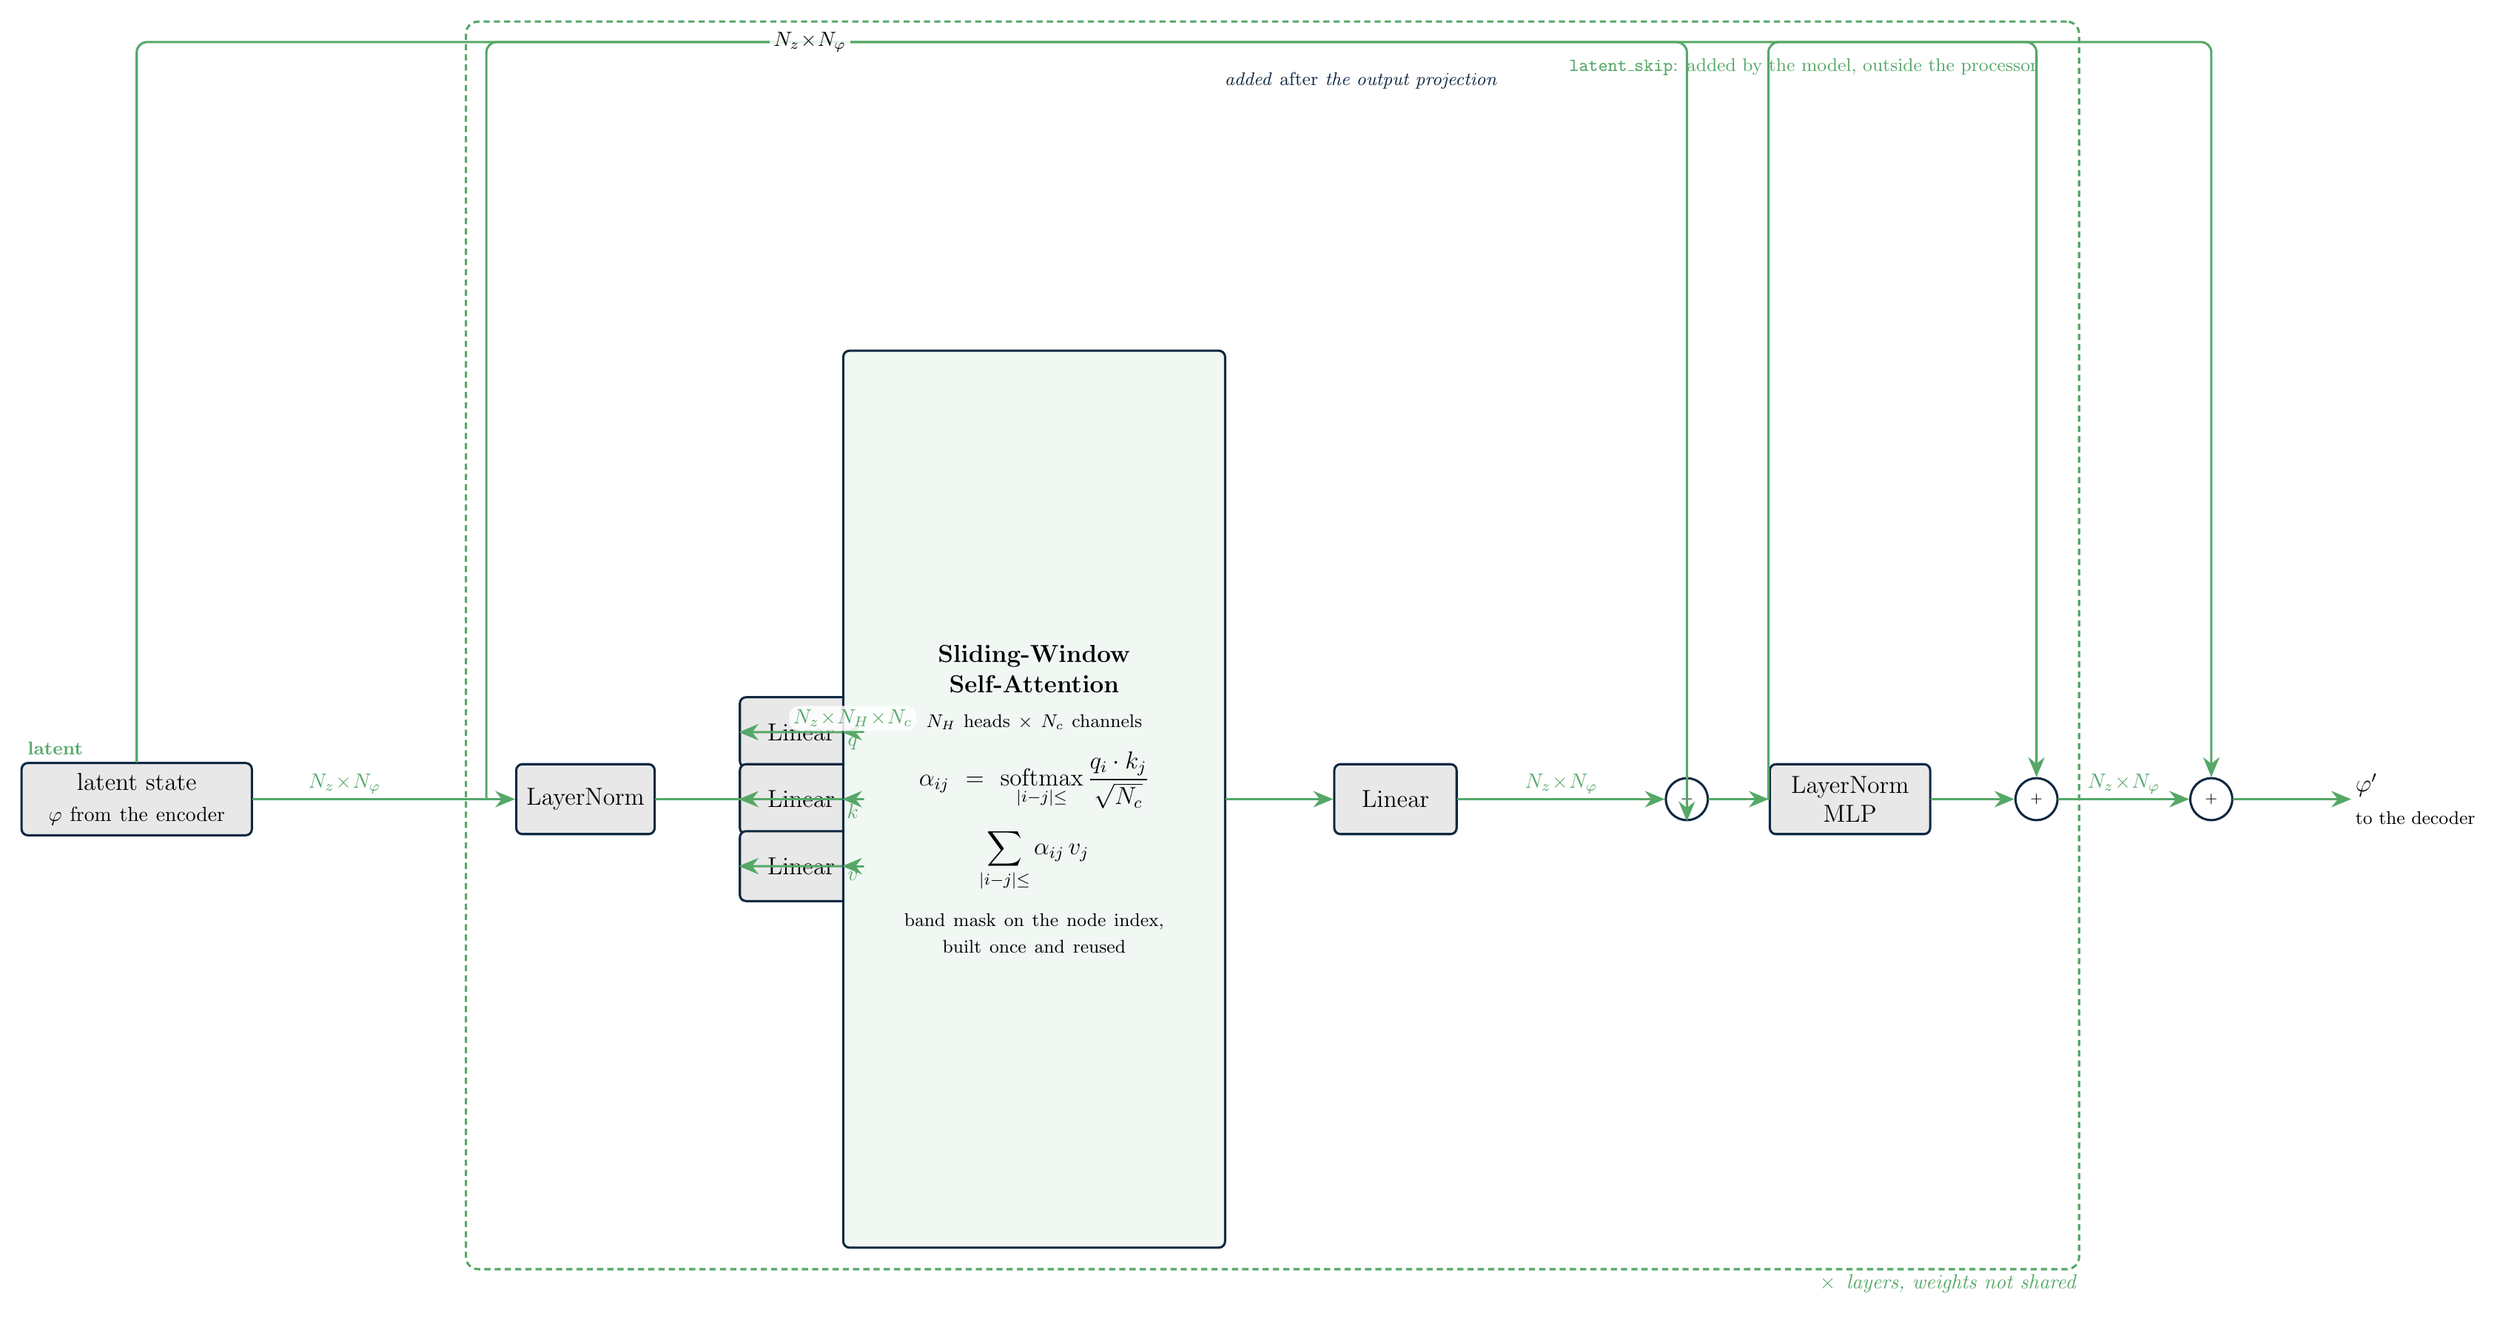
\begin{tikzpicture}[
  x=1cm, y=1cm, font=\large,
  blk/.style     = {rounded corners=3pt, draw=trapline, fill=trapfill,
                    line width=1.1pt, align=center, inner sep=5pt,
                    minimum height=1.2cm, minimum width=2.1cm},
  attnblk/.style = {blk, fill=attnfill},
  sum/.style     = {circle, draw=trapline, fill=white, line width=1.1pt,
                    inner sep=0pt, minimum size=0.72cm},
  term/.style    = {align=center, inner sep=2pt},
  wire/.style    = {-{Stealth[length=3.4mm,width=2.8mm]}, line width=1.1pt,
                    line cap=round, rounded corners=5pt},
  plain/.style   = {line width=1.1pt, line cap=round, rounded corners=5pt},
  shp/.style     = {font=\normalsize, inner sep=2pt, fill=white,
                    fill opacity=0.85, text opacity=1},
  tag/.style     = {font=\normalsize\itshape, inner sep=2pt},
  lane/.style    = {font=\small\bfseries, anchor=south west},
  repeat/.style  = {draw=latentclr, densely dashed, line width=1.1pt,
                    rounded corners=6pt, inner sep=10pt},
]

% =========================== INPUT ==========================================
\node[blk, text width=3.6cm] (phin) at (\colA, \rowlat)
  {latent state\\[1pt]{\normalsize$\latentvec$ from the encoder}};
\node[lane, text=latentclr, anchor=south west] at (phin.north west) {latent};

% =========================== ATTENTION SUBLAYER =============================
\node[blk] (lna)  at (\colB, \rowlat) {LayerNorm};
\node[blk] (linq) at (\colC, {\rowlat+\stack}) {Linear};
\node[blk] (link) at (\colC, \rowlat)          {Linear};
\node[blk] (linv) at (\colC, {\rowlat-\stack}) {Linear};
\coordinate (fan) at (\colsplit, \rowlat);

\coordinate (blockin) at ({\colB-1.7}, \rowlat);
\draw[wire, latentclr] (phin) -- node[shp, above, pos=0.35] {\shapetwo{\Nz}{\Nphi}} (lna);
\draw[plain, latentclr] (lna.east) -- (fan);
\draw[wire, latentclr] (fan) |- (linq.west);
\draw[wire, latentclr] (fan) -- (link.west);
\draw[wire, latentclr] (fan) |- (linv.west);

\node[attnblk, minimum height=15.4cm, text width=6.2cm] (attn) at (\colD, \rowlat)
  {\textbf{Sliding-Window}\\[1pt]\textbf{Self-Attention}\\[3pt]
   {\small $\NH$ heads $\times$ $\Nc$ channels}\\[10pt]
   {\large$\displaystyle
      \attn_{ij}=\operatorname*{softmax}_{|i-j|\le\Nw}
      \frac{\query_i\cdot\keyv_j}{\sqrt{\Nc}}$}\\[9pt]
   {\large$\displaystyle\sum_{|i-j|\le\Nw}\attn_{ij}\,\valuev_j$}\\[10pt]
   {\small band mask on the node index,\\[-1pt]built once and reused}};

\draw[wire, latentclr] (linq.east) -- node[shp, above]
  {\shapethree{\Nz}{\NH}{\Nc}} node[tag, below, text=latentclr] {$\query$}
  (linq.east -| attn.west);
\draw[wire, latentclr] (link.east) -- node[tag, below, text=latentclr] {$\keyv$}
  (link.east -| attn.west);
\draw[wire, latentclr] (linv.east) -- node[tag, below, text=latentclr] {$\valuev$}
  (linv.east -| attn.west);

\node[blk] (proj) at (\colE, \rowlat) {Linear};
\node[sum] (res1) at (\colF, \rowlat) {\scriptsize$+$};
\draw[wire, latentclr] (attn.east) -- (proj);
\draw[wire, latentclr] (proj) -- node[shp, above] {\shapetwo{\Nz}{\Nphi}} (res1);

% pre-norm skip around the whole attention sublayer, added AFTER the output
% projection -- the standard transformer arrangement, and not what the two
% mappers do with their lin_self branch
\coordinate (attnskipturn) at ({\colF}, \rowattnskip);
\draw[wire, latentclr] (blockin) |- (attnskipturn) -- (res1.south);
\node[tag, text=trapline, align=center, anchor=north]
  at ({(\colD+\colF)/2}, {\rowattnskip+0.55})
  {\small added \emph{after} the output projection};

% =========================== MLP SUBLAYER ===================================
\node[blk, text width=2.4cm] (ff)  at (\colG, \rowlat) {LayerNorm\\MLP};
\node[sum]                   (res2) at (\colH, \rowlat) {\scriptsize$+$};
\draw[wire, latentclr] (res1) -- (ff);
\draw[wire, latentclr] (ff) -- (res2);
\coordinate (mlpskipturn) at ({\colH}, \rowmlpskip);
\draw[wire, latentclr] ({(\colF+\colG)/2}, \rowlat) |- (mlpskipturn)
  -- (res2.north);

% =========================== REPEAT + OUTPUT ================================
\node[repeat, fit=(blockin) (lna) (linq) (linv) (attn) (res2)
                   (attnskipturn) (mlpskipturn)] (layer) {};
\node[tag, text=latentclr, anchor=north east] at (layer.south east)
  {$\times\,\NL$ layers, weights not shared};

\node[sum] (skipadd) at (\colI, \rowlat) {\scriptsize$+$};
\node[term, anchor=west, align=left] (out) at ({\colI+2.4}, \rowlat)
  {$\latentvec'$\\[2pt]{\small to the decoder}};
\draw[wire, latentclr] (res2) -- node[shp, above] {\shapetwo{\Nz}{\Nphi}} (skipadd);
\draw[wire, latentclr] (skipadd) -- (out);

% the model's own latent skip, outside the layer stack: x_latent_proc + x_latent
\draw[wire, latentclr] (phin.north) |- ({\colI}, \rowskip) -- (skipadd.north);
\node[shp] at ({(\colB+\colD)/2}, \rowskip) {\shapetwo{\Nz}{\Nphi}};
\node[term, anchor=south, align=center, font=\small, text=latentclr]
  at ({(\colE+\colI)/2}, {\rowskip+0.35})
  {{\tt latent\_skip}: added by the model, outside the processor};

\end{tikzpicture}
}
\end{center}
\vspace*{\fill}

{\footnotesize
    \textbf{Processor.}\;
    \texttt{TransformerProcessor} --- $\NL$ blocks over the latent nodes alone,
    with separate weights, and the only stage of the model that is not a graph
    operation.  The processor's graph provider is a \texttt{NoOpGraphProvider}
    and \texttt{TransformerProcessor} accepts \texttt{edge\_attr} and
    \texttt{edge\_index} only to discard them
    (\texttt{processor.py:298--316}), so the hidden-to-hidden graph plays no part
    and there is no edge lane to draw.
    Attention is instead a band on the node \emph{index}: the mask is
    $|i-j|\le\Nw$, built once on the first forward pass and reused.  Because the
    hidden nodes are HEALPix in \emph{ring} order
    (\texttt{nest\_ordering: false}), consecutive indices run along a latitude
    ring, so that band is a zonal strip --- every longitude, about
    \valwindowlat\textdegree\ of latitude --- rather than a compact patch.
    Each block is the standard pre-norm transformer arrangement, and differs from
    the two mappers in where its residual lands: here it is added \emph{after}
    the output projection, where the mappers add their $\selfv$ branch before it.
    The \texttt{latent\_skip} add on the right belongs to the model rather than to
    the processor.
\par}

\clearpage

% ============================== page 3 =====================================
\vspace*{\fill}
\begin{center}
  \resizebox{\textwidth}{!}{% ---------------------------------------------------------------------------
% Decoder of AnemoiModelEncProcDec (GraphTransformerBackwardMapper), drawn to
% match encoder_figure.tex block for block.
%
% The tikzpicture only -- \input it into a document whose preamble loads
% notation.tex and the tikz libraries listed in network_diagram.tex.
%
% Lane convention is shared with the encoder page: the SOURCE lane is on top and
% supplies key and value, the edge lane is in the middle, the DESTINATION lane is
% at the bottom and supplies query and self, and the destination stream leaves
% along the middle line.  The encoder and the decoder therefore have the same
% shape; only the colours swap, because the two spaces have swapped roles --
%   encoder:  source = data (blue),   destination = latent (green)
%   decoder:  source = latent (green), destination = data (blue)
%
% Two things differ structurally from the encoder and both are drawn:
%   1. there is no source embedding -- the mapper has no emb_nodes_src, so the
%      latent state enters the LayerNorm directly (mapper.py:698-701);
%   2. post_process is not the identity -- node_data_extractor, a LayerNorm and a
%      Linear, projects the latent width down onto the model's output channels
%      (mapper.py:688-705).  That Linear is where the diagnostic appears.
%
% Every node is placed off the \row*/\col* registers below, so the figure is
% reflowed by editing numbers in one place rather than by moving nodes.
% ---------------------------------------------------------------------------

% --- lane (row) positions ---------------------------------------------------
% The decoder chain is longer than the encoder's -- it carries the extractor and
% the residual add past the point where the encoder stops -- so the lanes are
% spread further apart than the encoder's to keep the aspect ratio near 1.8:1.
% Apparent text size is set by that ratio, not by the font size, because the
% figure is placed with \resizebox{\textwidth}{!}.
\def\rowlat{0}           % latent-space lane -- the source here
\def\rowedge{-7.0}       % edge lane; also the data stream after attention
\def\rowdata{-14.0}      % data-space lane -- the destination here
\def\rowskip{5.0}        % raw input state running over the top to the residual add
\def\rowconn{-10.4}      % graph connectivity entering the attention block
\def\rowselfskip{-18.5}  % self branch routed under the attention block
\def\rowdstskip{-21.5}   % pre-norm destination skip routed under everything
\def\rowffskip{-3.6}     % skip around the feed forward

% --- column positions -------------------------------------------------------
\def\colA{0}        % inputs
\def\colB{6.2}      % embedding Linear (destination lane only)
\def\colC{10.6}     % LayerNorm
\def\colD{13.6}     % q / k / v / edge projections
\def\colsplit{12.3} % where a LayerNorm output branches in two
\def\colE{19.8}     % graph attention
\def\colF{24.8}     % residual 1
\def\colG{27.4}     % projection
\def\colH{30.4}     % residual 2
\def\colI{33.4}     % LayerNorm + feed forward
\def\colJ{36.2}     % residual 3
\def\colK{39.4}     % node_data_extractor
\def\colL{42.8}     % residual add on the prognostic channels
\def\colM{44.8}     % output

\def\stack{1.15}    % vertical offset of paired sub-boxes

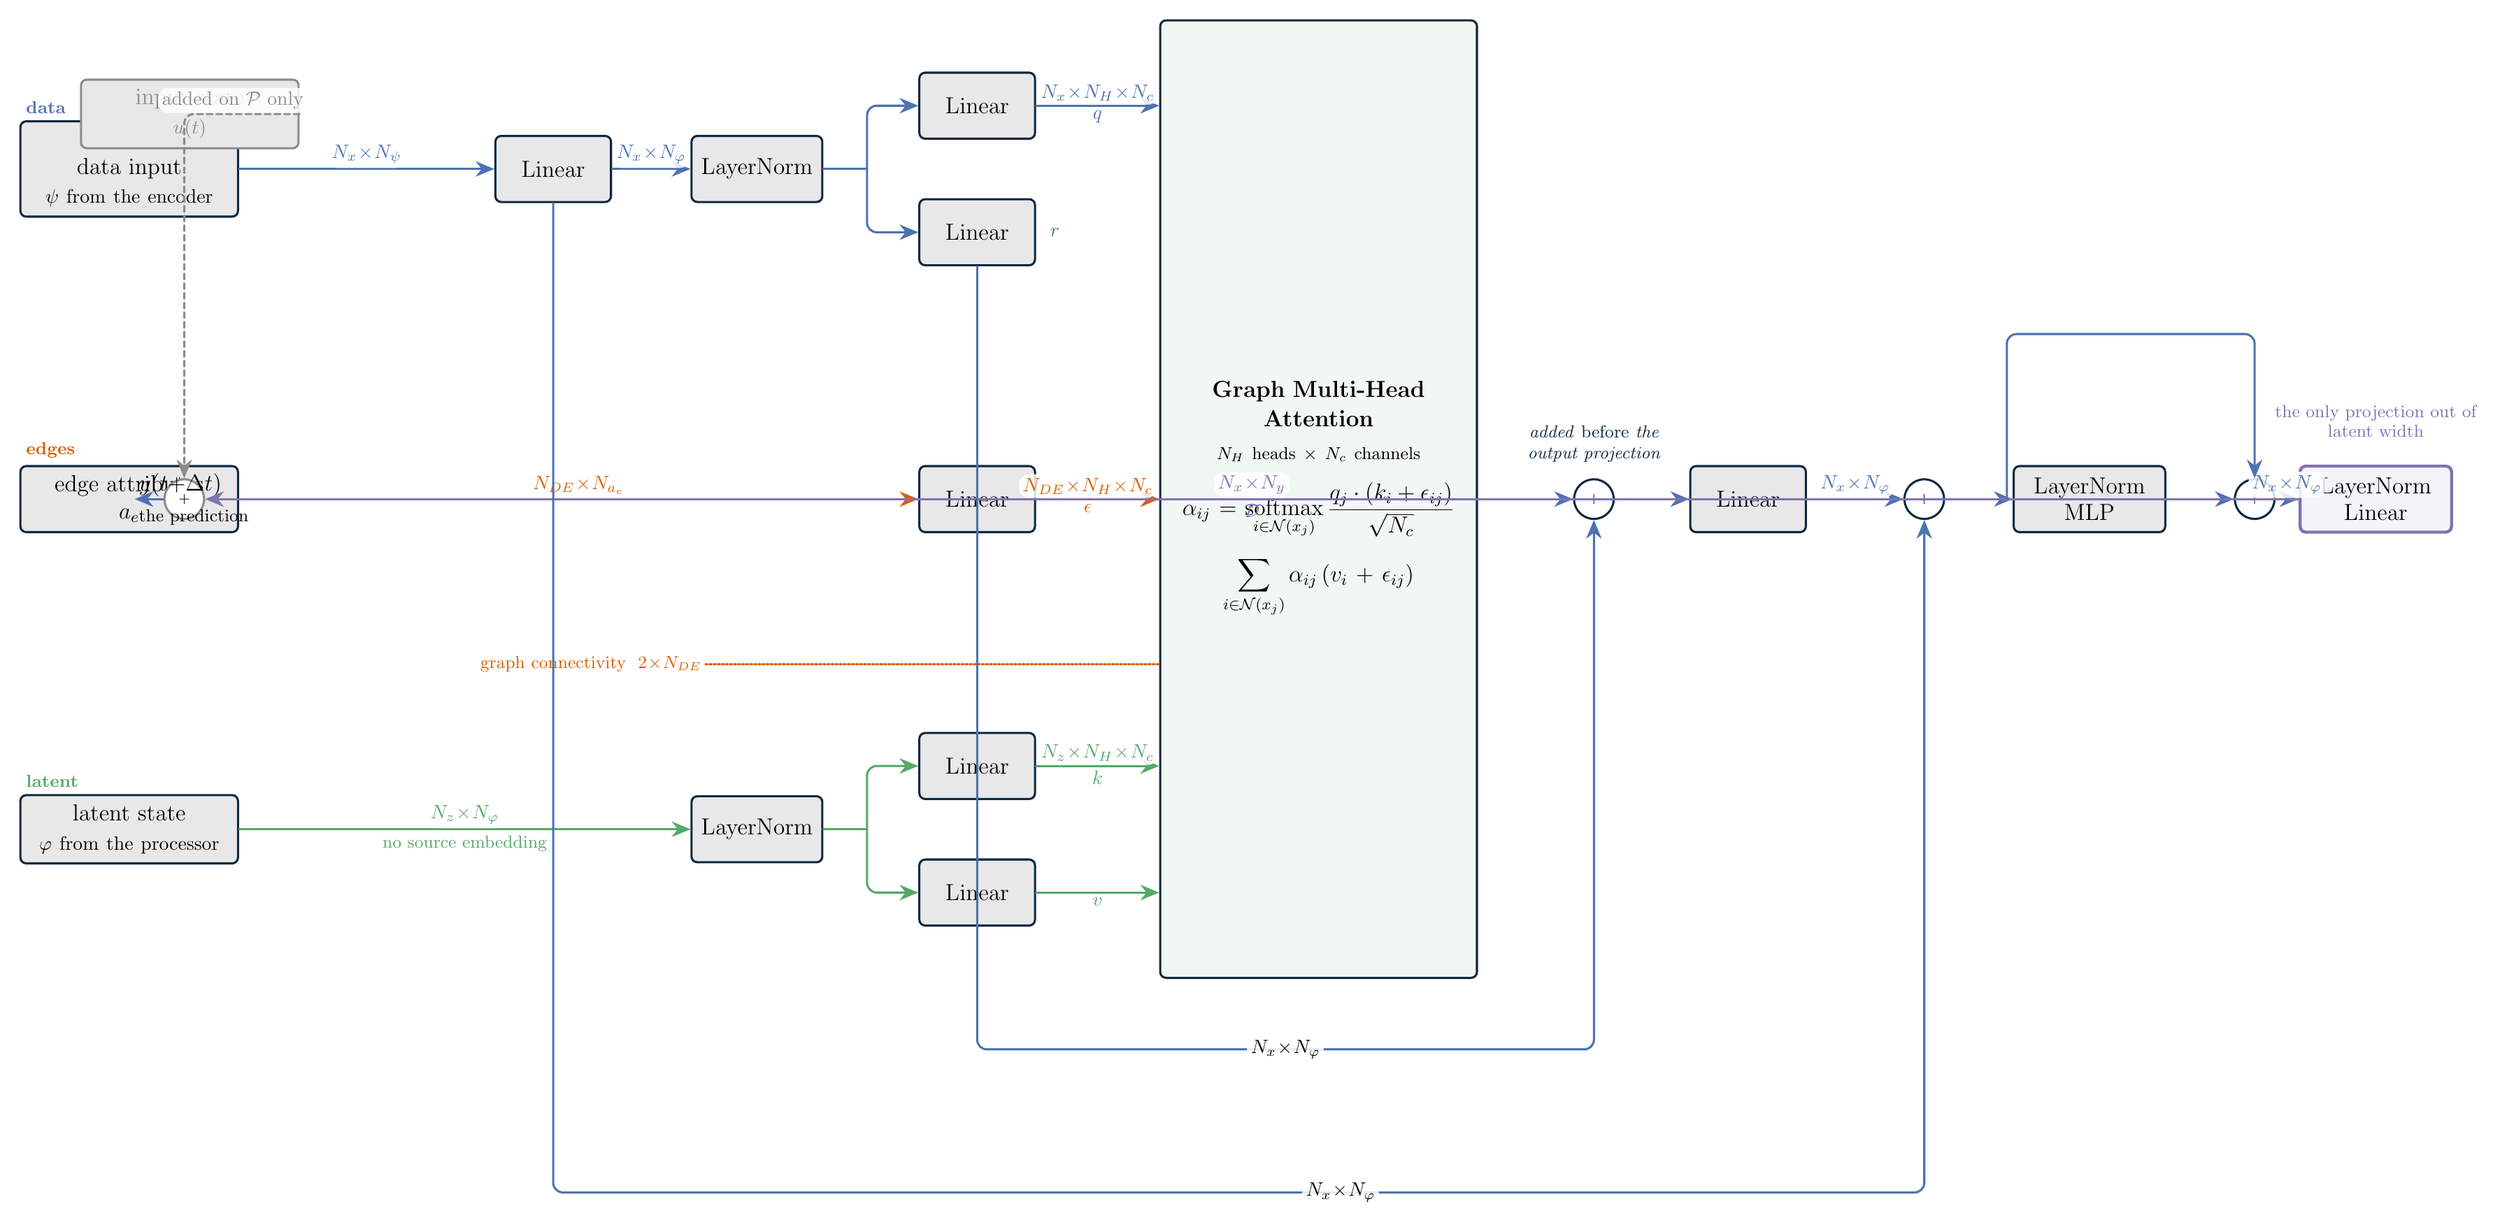
\begin{tikzpicture}[
  x=1cm, y=1cm, font=\large,
  blk/.style     = {rounded corners=3pt, draw=trapline, fill=trapfill,
                    line width=1.1pt, align=center, inner sep=5pt,
                    minimum height=1.2cm, minimum width=2.1cm},
  attnblk/.style = {blk, fill=attnfill},
  diagblk/.style = {blk, draw=diagclr, fill=diagfill, line width=1.6pt},
  sum/.style     = {circle, draw=trapline, fill=white, line width=1.1pt,
                    inner sep=0pt, minimum size=0.72cm},
  deadsum/.style = {sum, draw=inactiveclr},
  term/.style    = {align=center, inner sep=2pt},
  wire/.style    = {-{Stealth[length=3.4mm,width=2.8mm]}, line width=1.1pt,
                    line cap=round, rounded corners=5pt},
  plain/.style   = {line width=1.1pt, line cap=round, rounded corners=5pt},
  shp/.style     = {font=\normalsize, inner sep=2pt, fill=white,
                    fill opacity=0.85, text opacity=1},
  tag/.style     = {font=\normalsize\itshape, inner sep=2pt},
  lane/.style    = {font=\small\bfseries, anchor=south west},
]

% =========================== LATENT LANE (source) ===========================
% No embedding Linear: the backward mapper has no emb_nodes_src, so the
% processor's output enters the block's LayerNorm at its own width.
\node[blk, text width=3.6cm] (phin) at (\colA, \rowlat)
  {latent state\\[1pt]{\normalsize$\latentvec$ from the processor}};
\node[lane, text=latentclr, anchor=south west] at (phin.north west) {latent};
\node[blk] (lnz)  at (\colC, \rowlat) {LayerNorm};
\node[blk] (link) at (\colD, {\rowlat+\stack}) {Linear};
\node[blk] (linv) at (\colD, {\rowlat-\stack}) {Linear};
\coordinate (zsplit) at (\colsplit, \rowlat);

\draw[wire, latentclr] (phin) -- node[shp, above] {\shapetwo{\Nz}{\Nphi}}
  node[term, below, font=\small, text=latentclr, align=center, yshift=-1pt]
  {no source embedding} (lnz);
\draw[plain, latentclr] (lnz.east) -- (zsplit);
\draw[wire, latentclr] (zsplit) |- (link.west);
\draw[wire, latentclr] (zsplit) |- (linv.west);

% =========================== EDGE LANE ======================================
\node[blk, text width=3.6cm] (aein) at (\colA, \rowedge)
  {edge attributes\\$\attre$};
\node[lane, text=edgeclr, anchor=south west] at (aein.north west) {edges};
\node[blk] (line) at (\colD, \rowedge) {Linear};
\node[term, anchor=west, align=left, font=\small, text=edgeclr,
      fill=white, inner sep=2pt] (conn)
  at ({\colB-1.4}, \rowconn) {graph connectivity\ \ $2\!\times\!\NDE$};

\draw[wire, edgeclr] (aein) -- node[shp, above] {\shapetwo{\NDE}{\Nae}} (line);

% =========================== DATA LANE (destination) ========================
\node[blk, text width=3.6cm] (psiin) at (\colA, \rowdata)
  {assembled data input\\[1pt]{\normalsize$\inputvec$ from the encoder}};
\node[lane, text=dataclr, anchor=south west] at (psiin.north west) {data};
\node[blk] (embx) at (\colB, \rowdata) {Linear};
\node[blk] (lnx)  at (\colC, \rowdata) {LayerNorm};
\node[blk] (linq) at (\colD, {\rowdata+\stack}) {Linear};
\node[blk] (lins) at (\colD, {\rowdata-\stack}) {Linear};
\coordinate (xsplit) at (\colsplit, \rowdata);

\draw[wire, dataclr] (psiin) -- node[shp, above] {\shapetwo{\Nx}{\Npsi}} (embx);
\draw[wire, dataclr] (embx) -- node[shp, above] {\shapetwo{\Nx}{\Nphi}} (lnx);
\draw[plain, dataclr] (lnx.east) -- (xsplit);
\draw[wire, dataclr] (xsplit) |- (linq.west);
\draw[wire, dataclr] (xsplit) |- (lins.west);

% =========================== ATTENTION ======================================
\node[attnblk, minimum height=17.4cm, text width=5.4cm] (attn) at (\colE, \rowedge)
  {\textbf{Graph Multi-Head}\\[1pt]\textbf{Attention}\\[3pt]
   {\small $\NH$ heads $\times$ $\Nc$ channels}\\[10pt]
   {\large$\displaystyle
      \attn_{ij}=\operatorname*{softmax}_{i\in\nbhd(\coordx_j)}
      \frac{\query_j\cdot(\keyv_i+\edgeemb_{ij})}{\sqrt{\Nc}}$}\\[9pt]
   {\large$\displaystyle
      \sum_{i\in\nbhd(\coordx_j)}\attn_{ij}\,(\valuev_i+\edgeemb_{ij})$}};

\draw[wire, latentclr] (link.east) -- node[shp, above]
  {\shapethree{\Nz}{\NH}{\Nc}} node[tag, below, text=latentclr] {$\keyv$}
  (link.east -| attn.west);
\draw[wire, latentclr] (linv.east) -- node[tag, below, text=latentclr] {$\valuev$}
  (linv.east -| attn.west);
\draw[wire, edgeclr] (line.east) -- node[shp, above, pos=0.42]
  {\shapethree{\NDE}{\NH}{\Nc}} node[tag, below, pos=0.42, text=edgeclr] {$\edgeemb$}
  (line.east -| attn.west);
\draw[wire, dataclr] (linq.east) -- node[shp, above]
  {\shapethree{\Nx}{\NH}{\Nc}} node[tag, below, text=dataclr] {$\query$}
  (linq.east -| attn.west);
\draw[plain, edgeclr, densely dotted] (conn.east) -- (conn.east -| attn.west);

% =========================== POST-ATTENTION CHAIN ===========================
\node[sum] (res1) at (\colF, \rowedge) {\scriptsize$+$};
\node[blk] (proj) at (\colG, \rowedge) {Linear};
\node[sum] (res2) at (\colH, \rowedge) {\scriptsize$+$};
\node[blk, text width=2.4cm] (ff) at (\colI, \rowedge) {LayerNorm\\MLP};
\node[sum] (res3) at (\colJ, \rowedge) {\scriptsize$+$};
\node[diagblk, text width=2.4cm] (extract) at (\colK, \rowedge)
  {LayerNorm\\Linear};
\node[deadsum] (resprog) at (\colL, \rowedge) {\scriptsize$+$};
\node[term, anchor=west, align=left] (out) at ({\colM+0.1}, \rowedge)
  {$\outvec(t{+}\Delta t)$\\[2pt]{\small the prediction}};

\draw[wire, dataclr] (attn.east) -- (res1);
\draw[wire, dataclr] (res1) -- (proj);
\node[tag, above=6pt of res1, text=trapline, align=center]
  {\small added \emph{before} the\\[-1pt]\small output projection};
\draw[wire, dataclr] (proj) -- node[shp, above] {\shapetwo{\Nx}{\Nphi}} (res2);
\draw[wire, dataclr] (res2) -- (ff);
\draw[wire, dataclr] (ff) -- (res3);
\draw[wire, dataclr] (res3) -- node[shp, above] {\shapetwo{\Nx}{\Nphi}} (extract);
\draw[wire, diagclr] (extract) -- node[shp, above] {\shapetwo{\Nx}{\Nout}}
  node[tag, below, text=diagclr] {$\idxdiag$} (resprog);
\draw[wire, dataclr] (resprog) -- (out);

% residual 1 -- the self branch, added in attention space, ahead of the
% output projection (AIAYN draws that projection inside its attention box)
\draw[wire, dataclr] (lins.south) |- ({\colF}, \rowselfskip) -- (res1.south);
\node[shp] at ({(\colD+\colF)/2}, \rowselfskip) {\shapetwo{\Nx}{\Nphi}};
\node[tag, anchor=west, text=dataclr]
  at ({\colD+1.25}, {\rowdata-\stack}) {$\selfv$};

% residual 2 -- pre-norm skip taken from the data embedding
\draw[wire, dataclr] (embx.south) |- ({\colH}, \rowdstskip) -- (res2.south);
\node[shp] at ({(\colC+\colH)/2}, \rowdstskip) {\shapetwo{\Nx}{\Nphi}};

% residual 3 -- pre-norm skip around the MLP
\draw[wire, dataclr] ({(\colH+\colI)/2}, \rowedge) |- ({\colJ}, \rowffskip)
  -- (res3.north);

% =========================== OUTPUT =========================================
% node_data_extractor is the only place the network leaves latent width; its
% output columns are the model's output channels.  Which of those columns the
% residual add reaches -- prognostic only -- is what separates prognostic from
% diagnostic, and there is no diagnostic branch anywhere to draw.  See the Notes
% section of network_diagram.tex.
\node[term, anchor=south, align=center, text=diagclr, font=\small]
  at ({\colK}, {\rowedge+1.05})
  {the only projection out of\\[-1pt]latent width};

% the state-persistence residual, which reaches the prognostic channels only.
% Drawn grey and dashed: here that index set is empty.
\node[blk, text width=3.6cm, draw=inactiveclr, text=inactiveclr]
  (skipin) at ({\colA+1.1}, \rowskip)
  {input state\\[1pt]{\normalsize$\datavec(t)$}};
\draw[wire, inactiveclr, densely dashed] (skipin.east) -- ({\colL}, \rowskip)
  node[shp, above, pos=0.58, text=inactiveclr]
  {added on $\idxprog$ only} -- (resprog.north);

\end{tikzpicture}
}
\end{center}
\vspace*{\fill}

{\footnotesize
    \textbf{Decoder.}\;
    \texttt{GraphTransformerBackwardMapper} maps the processed latent mesh back
    onto the data nodes. It is the same block as the encoder with the two spaces
    exchanged: latent is now the source and supplies $\keyv$ and $\valuev$,
    whereas data is the destination, supplying $\query$ and $\selfv$.
    The three residual paths act on the destination path (latent lane in the encoder,
    data lane here).
    Two things are genuinely different from the encoder.
    First, there is no source embedding: the mapper defines only
    \texttt{emb\_nodes\_dst}, so $\latentvec$ enters the block at its own width
    while the destination input is embedded by a Linear of the decoder's own
    (\texttt{mapper.py:698--701}). That destination input is the raw
    $\inputvec$ handed back unchanged by the encoder, so the data-space input is
    embedded twice, by two independent matrices.
    Second, \texttt{post\_process} is not the identity: a LayerNorm and a Linear
    (\texttt{node\_data\_extractor}) take the latent width down to the
    model's $\Nout$ output channels. That Linear is the only place in the
    network that leaves latent width, and its output columns are the model
    output, which partitions into prognostic ($\idxprog$) and diagnostic
    ($\idxdiag$). Prognostic channels
    are also model inputs and are predicted as an increment on the last input
    step, which \texttt{\_assemble\_output} adds back; diagnostic channels are
    not inputs and receive no such add. Currently $\idxprog = \varnothing$.
\par}

\clearpage

% ============================== page 4 =====================================
\begin{center}
  \begin{minipage}{0.98\textwidth}
    \section*{Notation}

    Lowercase letters denote variables and functions; integer counts are written
    $N_{\text{quantity}}$.  Values are read directly from the checkpoint by
    \texttt{extract\_dims.py}, so they cannot drift from the trained model.

    \medskip
    % Two tabulars side by side: one table tall enough to overflow the page is
    % shipped as an overfull box on a page of its own.  The split point is set in
    % extract_dims.py, so rows can be added without touching this file.
    \begin{minipage}[t]{0.49\textwidth}
      \vspace{0pt}
      \begin{tabular}{@{}l >{\raggedright\arraybackslash}p{6.4cm} r@{}}
        \toprule
        symbol & meaning & value \\
        \midrule
        \symbolrowsone
        \bottomrule
      \end{tabular}
    \end{minipage}\hfill
    \begin{minipage}[t]{0.49\textwidth}
      \vspace{0pt}
      \begin{tabular}{@{}l >{\raggedright\arraybackslash}p{6.4cm} r@{}}
        \toprule
        symbol & meaning & value \\
        \midrule
        \symbolrowstwo
        \bottomrule
      \end{tabular}
    \end{minipage}

    \bigskip
    {\footnotesize
    $\|$ denotes concatenation along the feature axis.  \valtrainablenote\
    The encoder and the decoder run on different edge sets, with their own
    attributes and their own weights; $\attre$, $\Nae$, $\NH$, $\Nc$ and $\Nf$
    name the corresponding quantity in whichever of the two is being drawn.

    \smallskip
    Each latent node draws on a small local patch of the data mesh rather than
    on all of it: in this graph $\nbhd(\coordz_j)$ holds between \valdegmin\ and
    \valdegmax\ data nodes, \valdegmean\ on average.  It is empty for
    \valdegzero\ of the \valNz\ latent nodes, which by design receive no data
    and carry only their attributes and the skip connection into the processor.
    On the way back out the graph is a $k$-nearest-neighbour one rather than a
    cutoff, so $\nbhd(\coordx_j)$ \valdecdegphrase, for every one of the \valNx\
    data nodes.
    \par}
  \end{minipage}
\end{center}

\clearpage

% ============================== page 5 =====================================
% What this configuration is doing, as opposed to what the architecture could do.
% Anything that reads as "we could try X instead" belongs on page 5.
\section*{Notes}

\begin{minipage}{0.86\textwidth}
\small\sloppy
\begin{itemize}[leftmargin=1.1em]\setlength{\itemsep}{0.6em}

    \item \textbf{Currently, the only output is diagnostic, so the prognostic
        residual connection does nothing.}
      That is, $\idxprog = \varnothing$
      and $\idxdiag = \{\text{\tt sla}\}$.
      So, \texttt{SkipConnection} is instantiated and evaluated, and looks like
      a legitimate configuration turned on in the training yaml, but it does
      nothing.
      More importantly, the model has no direct persistence path, since the entire prediction
      comes from the extractor's Linear operation applied to the latent state.

      % This note is just for Claude, humans are well aware of it, but Claude
      % continues to rediscover this and raise it as an insightful finding.
      % Note: using nested ordering directly has undesirable effects that won't
      % be pursued unless explicitly asked to do so.
%    \item \textbf{The processor's attention window is a zonal band, not a
%      neighbourhood.}
%      \texttt{window\_size} is a half-width on the node \emph{index}, and the
%      hidden nodes are HEALPix in ring order, so index adjacency is longitude
%      adjacency along a latitude ring.  Measuring it on this graph:
%      $\Nw = \valNw$ spans about \valwindowlat\textdegree\ of latitude and every
%      longitude, several times over.  So a latent node attends zonally to the
%      whole globe but meridionally only $\pm$\,half that band, and with
%      $\NL = \valNL$ layers information cannot travel more than about
%      \valwindowreach\textdegree\ north or south in the entire processor.  For a global ocean
%      field that is a real anisotropy, and it is invisible in the config, which
%      just says \texttt{window\_size: \valNw}.  Switching the hidden nodes to
%      nested ordering, or dropping \texttt{window\_size} for global attention
%      over \valNz\ nodes, both change it.

\end{itemize}
\end{minipage}

\clearpage

% ============================== page 6 =====================================
% Points where these mappers depart from GraphCast-style message passing, from a
% plain GNN, or from a standard transformer.  Each is grounded in the source; the
% numbers come from dims.tex so they track the checkpoint.
\section*{Candidates for Architectural Experimentation}

{\small
Where these three stages depart from GraphCast-style message passing, from a
plain GNN, or from a standard transformer --- and what each departure might be
costing.  Line references are to \texttt{anemoi-core}; page 7 sets the same
departures against what GraphCast, GenCast and WeatherNext~2 actually do.
\par}

\begin{multicols}{3}
\footnotesize\sloppy  % narrow columns; prefer loose lines over overfull ones
\begin{itemize}[leftmargin=1.1em]\setlength{\itemsep}{0.35em}

    \item \textbf{Aggregation is degree-normalised; GraphCast's is not.}
      The softmax makes $\sum_{i\in\nbhd(\coordz_j)}\attn_{ij}=1$, so a latent
      node with one neighbour and one with fifteen both emit a unit-weight
      average.  GraphCast instead \emph{sums} MLP messages over incoming edges,
      so its aggregate grows with degree.  For a data-assimilation-like problem
      the observation density \emph{is} much of the signal, and here the
      attention output carries no magnitude cue for how well observed a patch
      is.  The \texttt{obs\_count} channels ride in $\inputvec$ and reach the
      values, but only indirectly.  GenCast and FGN divide by a constant, which is
      a resolution fix and not a degree normalisation: all three keep density in
      the magnitude.  Page 7.

    \item \textbf{Edge features are never updated.}
      GraphCast is an interaction network: each message-passing step rebuilds
      edge features from (sender, receiver, edge).  That bites in its
      \emph{processor}, which takes \gcsteps\ such steps; its mappers take one,
      and GenCast and FGN drop the edge residual there.  Here $\attre$ passes through
      one Linear into the keys and values and is returned unchanged
      (\texttt{block.py:1029}), then discarded by the mapper
      (\texttt{mapper.py:321}).  Edge geometry is a fixed bias, never a state, so
      it cannot be modulated by the flow it is carrying.

    \item \textbf{The edge embedding enters both the key and the value.}
      \texttt{conv.py:140} and \texttt{:147}, the same tensor twice.  Inherited
      from PyG's \texttt{TransformerConv} rather than invented here, and distinct
      both from GraphCast and from a plain transformer (page 7).  One
      \texttt{lin\_edge} is trained to do two different jobs: shift the logit and
      shift the payload.

    \item \textbf{There is no self-loop in the softmax.}
      In standard self-attention a token sits inside its own softmax, so
      own-state competes with neighbour-evidence on a normalised scale.  Here the
      node's own state re-enters outside the softmax,
      through $\selfv$.  The balance between own-state and neighbour-evidence is
      therefore set by the learned magnitude of \texttt{lin\_self} and is
      unbounded --- nothing stops it from swamping, or being swamped by, the
      aggregated data.  A property of the mappers only: our processor's band
      contains its own index, and GenCast adds self-loops deliberately.

    \item \textbf{The mappers and the processor disagree about where the
      residual goes.}
      \texttt{block.py:1017} computes \texttt{projection(out + x\_r)}, so in both
      mappers $\selfv$ is mixed by the output projection rather than added around
      it, and the genuine pre-norm residual is a separate add on the next line.
      The processor block does it the standard way,
      \texttt{x + attention(LayerNorm(x))}, with the add \emph{after} $W^O$.  One
      model, two conventions, and only the mappers' is unusual.

    \item \textbf{The decoder's destination input is raw, un-embedded $\inputvec$.}
      The forward mapper returns \texttt{x[0]} untouched
      (\texttt{mapper.py:597}), and the decoder re-embeds it with its own Linear.
      So \texttt{emb\_nodes\_src} serves the encoder's keys and values only and
      never reaches the decoder, and the data-space input is embedded twice by
      two independent matrices.  All three DeepMind models instead hand their
      decoder the \emph{encoded} grid latent, carried around the processor.  The
      clearest single ablation here.  Page 7.

    \item \textbf{The decoder has no source embedding at all.}
      \texttt{GraphTransformerBackwardMapper.pre\_process} embeds only the
      destination (\texttt{mapper.py:698--701}), so $\latentvec$ goes straight
      into the block's source LayerNorm.  Harmless while \texttt{num\_channels}
      is the width on both sides, but it means the latent stream gets no
      per-mapper reprojection on the way out --- the decoder's only chance to
      reweight latent channels before attending is the \texttt{lin\_key} /
      \texttt{lin\_value} pair.

    \item \textbf{The way out is $k$-nearest-neighbour, the way in is a cutoff.}
      Every data node attends to exactly \valdecdegmax\ latent nodes, whatever
      the local latent density, while a latent node gathers from between
      \valdegmin\ and \valdegmax\ data nodes.  The decoder's softmax therefore
      normalises over a fixed and very small set --- three logits, one head at a
      time, and a data node in a sparsely observed region is reconstructed from
      exactly as many latent nodes as one in a dense region.
      The \emph{count} is not the departure --- all three DeepMind models also read
      each grid node from exactly \dmdecdeg.  What differs is which three: theirs
      are the vertices of the containing triangle, so the node is guaranteed to sit
      inside the patch it reads from; ours are merely the nearest, which at a coast
      can all lie on one side.  Page 7.

    \item \textbf{Two places bypass \texttt{layer\_kernels}.}
      \texttt{node\_data\_extractor} is built from \texttt{nn.LayerNorm} and
      \texttt{nn.Linear} directly, and so are the processor's $\query$, $\keyv$
      and $\valuev$ projections (\texttt{attention.py:145--147}, which binds
      \texttt{layer\_kernels.Linear} and then uses it only for the output
      projection).  A change to \texttt{model.layer\_kernels} therefore silently
      misses both the layer that produces the model's output and three of the four
      Linears in every processor block.

    \item \textbf{\texttt{num\_chunks} means two different things.}
      In the mappers it partitions destination nodes for memory
      (\texttt{mapper.py:296}); in the processor it divides the layer stack into
      gradient-checkpointing groups of \texttt{num\_layers / num\_chunks}
      (\texttt{processor.py:90}).  Here $\valNchunk$ chunks over \valNL\ layers
      means one layer per checkpoint, i.e.\ maximum recomputation.

    \item \textbf{Nothing in this run is pinned to the graph --- but that is a
      config choice, not a property of the architecture.}
      Every \texttt{trainable\_size} is zero, so the node and edge attributes are
      purely geometric and the trainable node-plus-edge total is
      \valgraphparams\ against \valtotalparams\ in the model.  The stock anemoi
      configs instead give each node and each edge a zero-initialised trainable
      tail, costing order $\Nx+\Nz$ parameters for the nodes and $\NEE+\NDE$ for
      the edges, none of which transfer to another graph.  Worth suspecting first if spatial generalisation
      looks surprisingly good once they are turned on.  Note which side is unusual:
      no DeepMind model has a learned per-node or per-edge parameter at all, so
      zeroing them puts this run \emph{with} the lineage.

    \item \textbf{Depth is in the processor, not in the mappers.}
      \texttt{self.proc} is one \texttt{Graph\-Transformer\-Mapper\-Block} at
      each end, not a stack (\texttt{mapper.py:222}): \valencparams\ parameters
      in the encoder and \valdecparams\ in the decoder against \valprocparams\
      in the processor.  GraphCast's encoder is likewise one message-passing step,
      so this matches --- but with a one-hop neighbourhood at both ends the whole
      path from data to latent, and back, is a single local gather.

    \item \textbf{The residual branches could start at zero.}
      GenCast and FGN zero-initialise both output projections in every processor
      block, so the stack is an identity at initialisation; ours do not.  Page 7.

    \item \textbf{Multi-dataset latents are summed, not gated.}
      Every dataset contributes additively with no learned weighting, and each
      carries its own copy of the latent-attribute residual
      (\texttt{encoder\_\-processor\_\-decoder.py:273}).

\end{itemize}
\end{multicols}

\clearpage

% ============================== page 7 =====================================
% Where these three stages sit relative to GraphCast, GenCast and WeatherNext 2.
% Pages 5, 6 and 7 split as: what is true of this run / what to try / what someone
% else did.  Every DeepMind number here comes from deepmind.tex, which is
% hand-maintained and carries a provenance tag per value; every number of ours
% still comes from dims.tex.
\section*{Comparison with the DeepMind lineage}

{\small\sloppy
The three models are one codebase.  {\tt google-deepmind/graphcast} was renamed to
{\tt google-deepmind/weathernext}, and GraphCast, the GenCast denoiser and
FGN / WeatherNext~2 now sit side by side in {\tt weathernext1\_graph/},
{\tt weathernext1\_gen/} and {\tt weathernext2/} over a shared {\tt utils/} ---
GenCast and FGN import the same {\tt sparse\_transformer.py}, and FGN's own
appendix calls its architecture ``very similar to that of GenCast''.  Read in one
tree the shape of the lineage is plain: \textbf{the encoder and the decoder barely
changed across three models, and the processor is the only stage that was ever
redesigned.}
\par}

{\footnotesize\smallskip
Two differences are assumed throughout and not repeated below.  They train on full
gridded reanalysis or analysis fields, where we train on sparse per-mission
altimeter observations binned onto a sea-masked HEALPix grid.  And we are
deterministic with an MSE loss, so GenCast is taken here as its denoiser core
alone, as though it were deterministic, and FGN's noise mechanism is described
only where it changes which layers exist.
\par}

\smallskip
{\footnotesize
\begin{center}
\begin{tabular}{@{}l r r r r@{}}
  \toprule
   & GraphCast & GenCast & WN2 & here \\
  \midrule
  latent width      & \gclatent & \genlatent & \fgnlatent & \valNphi \\
  processor depth   & \gcsteps  & \genlayers & \fgnlayers & \valNL \\
  heads $\times$ ch.& ---       & $\genheads\!\times\!\genheaddim$
                                & $\fgnheads\!\times\!\fgnheaddim$
                                & $\valNH\!\times\!\valNc$ \\
  latent nodes      & \dmmeshnodes & \dmmeshnodes & \dmmeshnodes & \valNz \\
  parameters (M)    & \gcparams & $\sim$\genparams & $\sim$\fgnparams
                                & \valtotalparamsM \\
  \bottomrule
\end{tabular}
\end{center}
\par}

\medskip
\begin{multicols}{3}
\footnotesize\sloppy

\subsection*{Encoder}

\textit{GraphCast built the grid-to-mesh edges with a ball query at
\dmradiusfrac\ times the longest finest-mesh edge and ran one round of
interaction-network message passing.  GenCast kept both; FGN kept both.  Across
three models the only encoder changes were widths.}

\begin{itemize}[leftmargin=1.1em]\setlength{\itemsep}{0.45em}

  \item \textbf{Their query radius is tied to the mesh; ours is tied to
    kilometres.}  Theirs is \dmradiusfrac\ $\times$ the longest edge of the
    finest mesh --- about \dmradiuskm\,km at level \dmmeshlevel\ --- so it
    rescales itself whenever the mesh or the grid changes.  Measured on this
    graph, our longest surviving encoder edge is \valenccutoffkm\,km against a
    hidden-node spacing of \valhiddenspacing\,km, a ratio of
    \valcutoffratio\ where theirs is \dmradiusfrac.  Theirs is also chosen so
    that every grid node reaches at least one mesh node; ours is a cutoff, so
    $\nbhd(\coordz_j)$ is empty for \valdegzero\ latent nodes --- by design,
    from land masking.  Their in-degree is about \gcencdeg\ grid nodes per mesh
    node, ours \valdegmean.

  \item \textbf{They kept an aggregate that grows with degree, three times over.}
    GraphCast sums messages with no normalisation at all.  GenCast divides by a
    constant \genaggnorm\ and FGN by \fgnaggnorm\ --- and GenCast's
    \genaggnorm\ was introduced when they fine-tuned from 1\textdegree\ to
    0.25\textdegree, so each mesh node began receiving \genaggnorm$\times$ more
    messages.  That is a resolution scale fix, not a degree normalisation: all
    three still carry observation density in the magnitude.  Our softmax makes
    the aggregate degree-invariant.  See page 6.

  \item \textbf{Message form.}  Theirs is an interaction network:
    $\mathrm{MLP}([\attre, v_{\text{src}}, v_{\text{dst}}])$ summed into
    $\mathrm{MLP}([v_{\text{dst}}, \textstyle\sum])$, with residual adds on nodes
    \emph{and} on edges.  Ours is attention, with one {\tt lin\_edge} feeding both
    the key and the value.

  \item \textbf{Two norm conventions in one model is not unique to us.}  Their
    mappers are post-norm inside the residual branch,
    $x + \mathrm{LayerNorm}(\mathrm{MLP}(\cdot))$, while only their processor is
    pre-norm.  We differ in which stage gets which, not in being mixed.

  \item \textbf{Mesh-node inputs.}  All three give mesh nodes three geometric
    features and nothing else, zero-padded up to the grid width so one embedder
    serves both.  Ours gives latent nodes $\attrz$ and a Linear of its own ---
    the same idea without the padding trick.

\end{itemize}

\subsection*{Processor}

\textit{GraphCast ran \gcsteps\ message-passing steps over a multimesh, levels
\gcmeshlevels\ merged into one graph so that long edges existed explicitly.
GenCast deleted the multimesh and replaced the whole stage with \genlayers\
pre-norm transformer blocks on the finest mesh alone, sparsified by a $k$-hop
mask.  FGN kept that file unchanged and scaled it to \fgnlayers\ blocks.}

\begin{itemize}[leftmargin=1.1em]\setlength{\itemsep}{0.45em}

  \item \textbf{Their neighbourhood is $k$ hops on the mesh graph, not a radius.}
    The mask is literally {\tt mask = adj\_mat ** attention\_k\_hop}, a sparse
    matrix power of the mesh adjacency with self-loops, so node $i$ attends to
    $j$ exactly when a walk of at most $k$ mesh edges joins them.  With
    $k = \genkhop$ at level \dmmeshlevel\ that is \genballnodes\ of
    \dmmeshnodes\ nodes, and because the mesh is near-uniform it behaves like a
    geodesic disc of roughly \genballkm\,km --- isotropic by construction rather
    than by a metric query.  It is built once on the host and never
    recomputed.  Ours is a band on the node \emph{index} instead: the mask is
    $|i-j|\le\Nw$, and the graph plays no part in it.

  \item \textbf{The one axis on which we already match is density.}  Their ball
    is \gendensity\% of the mesh; our window is $2\Nw+1$ of \valNz\ nodes, or
    \valwindowfrac\%.  Nearly the same fraction of the mesh, arrived at
    independently and shaped differently.

  \item \textbf{They also permute the mesh to get a band --- in the other
    direction.}  A reverse Cuthill--McKee ordering is applied so that the
    \emph{graph} mask comes out banded and a block-sparse attention kernel can
    skip whole tiles.  The band is the optimisation; the graph is still the
    definition.

  \item \textbf{Both sides carry vestigial edge plumbing.}  GenCast computes mesh
    edge features and then discards them --- its {\tt MeshTransformer} reads node
    features and the edge \emph{indices} only.  Our {\tt NoOpGraphProvider} and
    the dropped {\tt edge\_attr} / {\tt edge\_index} reach the same place by a
    different route.

  \item \textbf{Conditional LayerNorm is the lineage's structural extension
    point.}  Both GenCast and FGN strip the learned scale and offset out of every
    LayerNorm and supply them from a FiLM layer driven by one global vector: the
    diffusion noise level in GenCast, a learned \fgnnoisedim-element noise vector
    in FGN, \fgnfilmlayers\ such layers in all.  Repointing that vector is
    essentially the whole architectural difference between the two.  Ours are
    stock {\tt torch.nn.LayerNorm} with their own affine, so there is no slot for
    a global signal --- worth knowing before a forcing, an analysis time or an
    observation-density summary needs somewhere to enter.

  \item \textbf{Their residual branches start at exactly zero.}  Both attention
    and MLP output projections are zero-initialised, so every block is an
    identity at initialisation and training begins from encoder-to-decoder alone.
    Ours use default {\tt torch} init; anemoi exposes
    {\tt initialise\_data\_extractor\_zero} for the decoder head and nothing
    equivalent for the processor.

\end{itemize}


\subsection*{Decoder}

\textit{GraphCast read each grid node from the three vertices of the mesh
triangle containing it, ran one message-passing step and a readout MLP, and fed
that decoder the \emph{encoder's} grid latent rather than the raw input.  GenCast
and FGN changed none of it.}

\begin{itemize}[leftmargin=1.1em]\setlength{\itemsep}{0.45em}

  \item \textbf{Three neighbours on the way out, in all four models.}  So the
    cardinality is not a departure --- page 6 previously read as though it were.
    The difference is what the three are: theirs are the vertices of the
    containing triangle, so the grid node is guaranteed to lie inside the patch
    it reads from, where our $k$-nearest-neighbour graph gives no such guarantee
    and can draw all \valdecdegmax\ from one side at a coast or a mask edge.

  \item \textbf{The long skip is the real gap.}  All three feed the decoder the
    encoder's grid latent --- embedded, message-passed, and carried around the
    entire processor --- so their decoder residual lands on a processed
    representation.  Ours feeds the raw un-embedded $\inputvec$, re-embedded by a
    second independent Linear.  This is the clearest single ablation on either
    page.

  \item \textbf{Their readout MLP deliberately has no LayerNorm.}  GraphCast
    states it outright --- every MLP is followed by a LayerNorm except the
    decoder's --- and FGN's grid decoder is the one module in the network with no
    FiLM.  Ours is {\tt LayerNorm} then {\tt Linear}, and is also the layer that
    bypasses {\tt layer\_kernels}.

  \item \textbf{Prognostic against diagnostic is the same index-set mechanism.}
    A target that also appears in the inputs is predicted as an increment on the
    last input step and added back; one that does not is predicted directly.  No
    separate branch, in their code or ours.  Their diagnostic is 6-hour
    precipitation, ours is {\tt sla}, and since $\idxprog = \varnothing$ we sit
    permanently in the ``predicted directly'' case.  Their increments are
    normalised by the per-variable, per-level standard deviation of the
    \emph{differences}, with the mean not subtracted.

\end{itemize}

\end{multicols}

\end{document}
